\section{Numerical results for fixed cooling times}\label{numerical}
This section investigates the linear growth of the VSI with fixed
cooling times, $\beta\OmK^{-1}$, that are independent of height.  
We solve the radially local model of Eqs.\ \ref{lin_all} with
$\zeta=1$, i.e.\ retaining  radial gradients of the background disk
structure. The equilbrium disk structure given is in \S\ref{eqm}. This
numerical study does not make the simplifying approximations  
used in \S\ref{analytical}. 

We solve the linear problem by expanding the 
perturbations in Chebyshev polynomials $T_l$ up to $l=512$
and discretizing the equations on a grid with
$z\in[-\zmax,\zmax]$. Our standard boundary conditions at the vertical
boundaries is a free surface,  
\begin{align}
  \Delta P \equiv \delta P + \bm{\xi}\cdot\nabla P= 0 \quad \text{at } z=\pm\zmax,
\end{align}
% note that there are g_c terms in the boundary condition
where $\bm{\xi}$ is the Lagrangian displacement with meridional 
components $\xi_{x,z} = \ii\delta v_{x,z}/\upsilon$. In some cases we
impose a rigid boundary with $\delta v_z(\pm\zmax)=0$. 

The above discretization procedure
converts the linear system of differential equations to a set of 
algebraic equations,  which we solve using LAPACK matrix
routines\footnote{Available at \url{http://www.netlib.org/lapack/}.}.  

Unless otherwise stated, we adopt fiducial disk parameters are 
$(\gamma, \Gamma) = (1.4, 1.011)$, $(p,q, h)=(-1.5,-1,0.05)$, and 
vertical domain size $\zmax=5H$. This setup is effectively vertically
isothermal since $c_s^2(\zmax) \simeq 0.9c_s^2(0)$.\footnote{While this model
has a zero density surface at $z = \pm H_s \simeq \pm 16.4 H$ (see Eq.\ \ref{eqm_rot}), the surface is 
outside the numerical domain.} In Fig. \ref{omega_z}
we plot the corresponding equilibrium rotation profile, which shows
that $\Omega$ decreases slightly away from the midplane.   From Eq.\ \ref{iso_vsi_cond},
we expect that $\beta < \beta_\mathrm{crit} = 0.125$ is needed for VSI growth in our fiducial model. 

\begin{figure}
  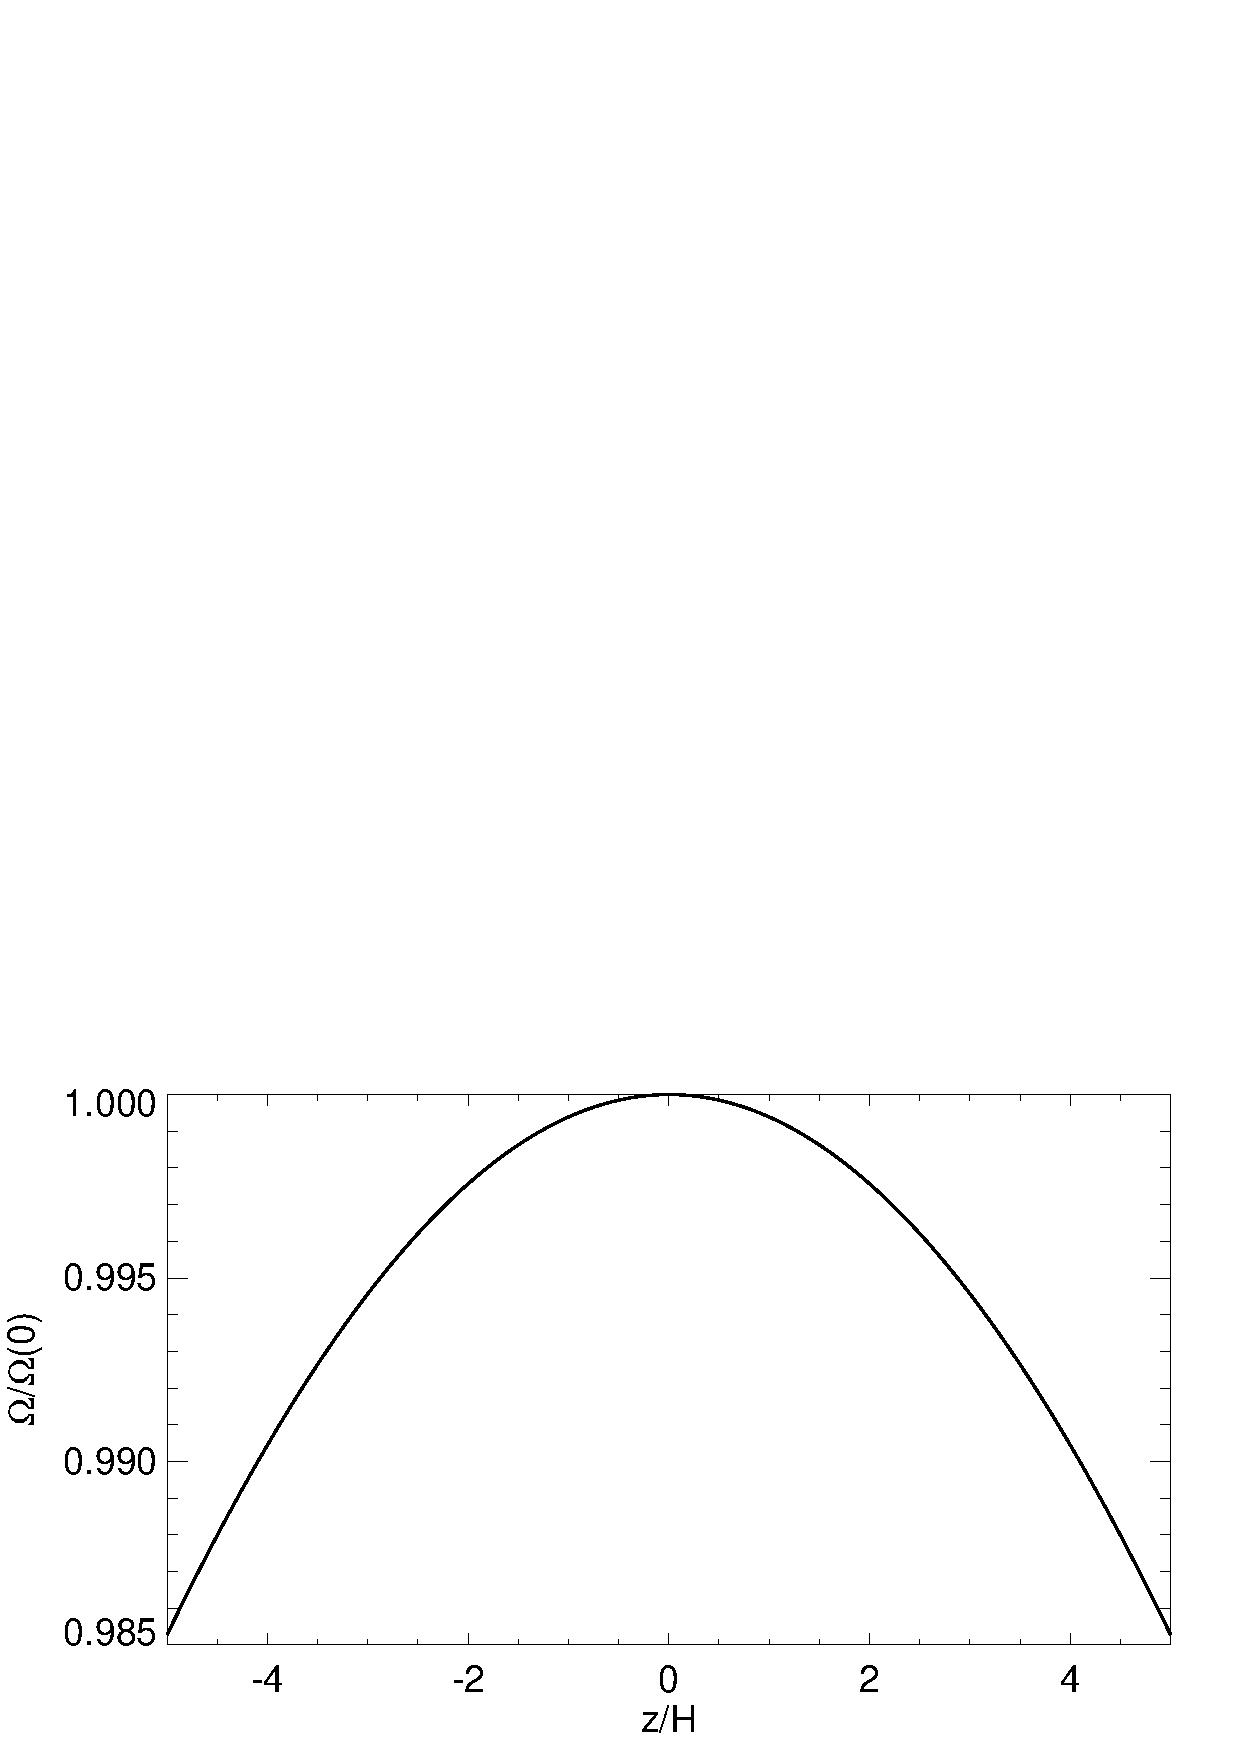
\includegraphics[width=\linewidth,clip=true,trim=0cm 0cm 0cm
  0cm]{figures/omega2} 
  \caption{Equilibrium rotation profile $\Omega(z)$,
    normalized by its mid-plane value, for  the fiducial disk model with $\Gamma=1.011$
    and $(p,q, h)=(-1.5,-1,0.05)$. 
    \label{omega_z} 
  }
\end{figure}

\begin{figure}
  \includegraphics[width=\linewidth]{figures/compare_modes_iso_kx10_analytic.ps}
  \caption{Growth rate, $\sigma$, vs.\ osciallation frequency, $\omega$, for
  VSI modes with wavenumber $k_x = \khat/H=10/H$ in the fiducial disk model
    with rapid cooling, $\beta=10^{-3}$. %  a disk with 
    % $(\gamma,\Gamma)=(1.4,1.011)$, $(p,q, h)=(-1.5,-1,0.1)$ and
    % $\beta=10^{-3}$. 
We investigate the effect of vertical box size, from $\zmax=3H$
(\emph{blue triangles}) to $7H$ (\emph{green} x's)
    with a free surface boundary ($\Delta P=0$).  For $\zmax=5H$  (black dots) we also compare free surface (\emph{black dots}) and rigid (\emph{red plusses}), finding little difference.
      The fundamental mode is marked by `f'. Lines show the analytic predictions for
      isothermal perturbations ($\beta = 0$, \emph{dashed}) and for $\beta = 10^{-3}$ (\emph{dotted}).
      See text for discussion.
   % are computed from the analytic dispersion relation 
    %with thermal relaxation Eq. \ref{relax_disp} (dotted), and that for
    %isothermal perturbations, Eq. \ref{simple_growth} (dashed). 
    \label{compare_modes_iso_kx10} 
  }
\end{figure}

\subsection{Rapid thermal relaxation}\label{vertiso_pertiso} 
We first calculate the VSI in a disk with rapid thermal relaxation by
setting $\beta=10^{-3}$.  Since $\beta \ll \beta_\mathrm{crit}$, this case
gives similar results to the well studied case of isothermal perturbations
 \citepalias[e.g.][]{nelson13,mcnally14,barker15}.\footnote{We confirmed that smaller
 $\beta$ values gave similar results.} This case allows us to explore and test our
finite cooling time model in a familiar context.

%For completeness, and as a way of introducing terminology, 
%we review this case before considering the effect of 
%thermal relaxation.\footnote{\emph{not accurate, even $\beta = 0$ is instant thermal relaxation...}} 

% Fig. \ref{iso_eigen_kx} compares the numerically obtained eigenvalues 
% for the fundamental mode and that calculated from 
% Eq. \ref{simple_growth}. We find good agreement in the
% wave frequency $\omega$ at all $\khat$ and in growth rates $\sigma$ for
% $\khat\gtrsim 10$. Growth rates are over-estimated by our analysis but 
% are $O( h\Omega_K)$, which is consistent with the discussion in
% Appendix \ref{max_growth1}. The match in $\sigma$ worsens for 
% decreasing $\khat$ due to the neglect of global radial structure in
% the analysis. Nevertheless, given the number of approximations made
% in our analysis, the agreement is satisfactory. 

% \begin{figure}
%   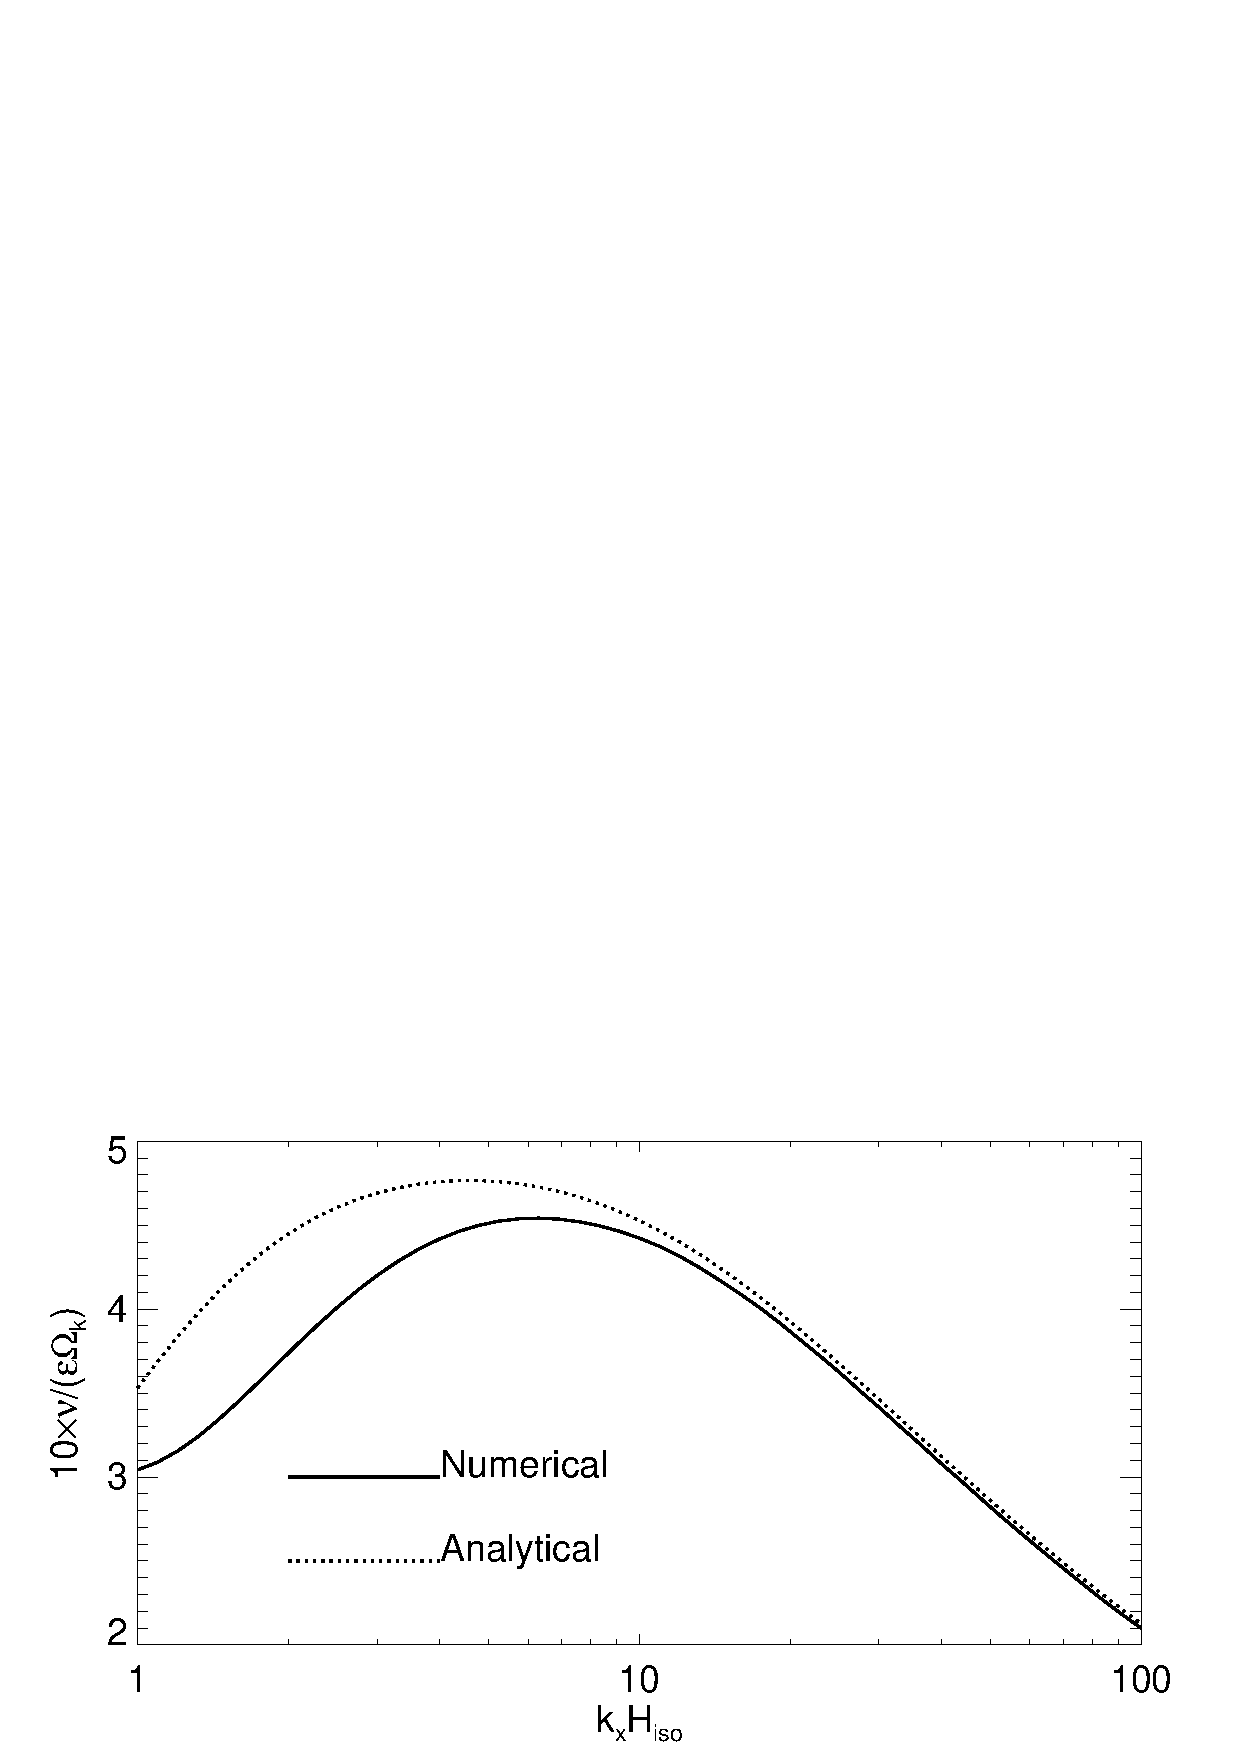
\includegraphics[width=\linewidth,clip=true,trim=0cm 1.75cm 0cm
%   0cm]{figures/compare_eigen_imag_iso} 
%   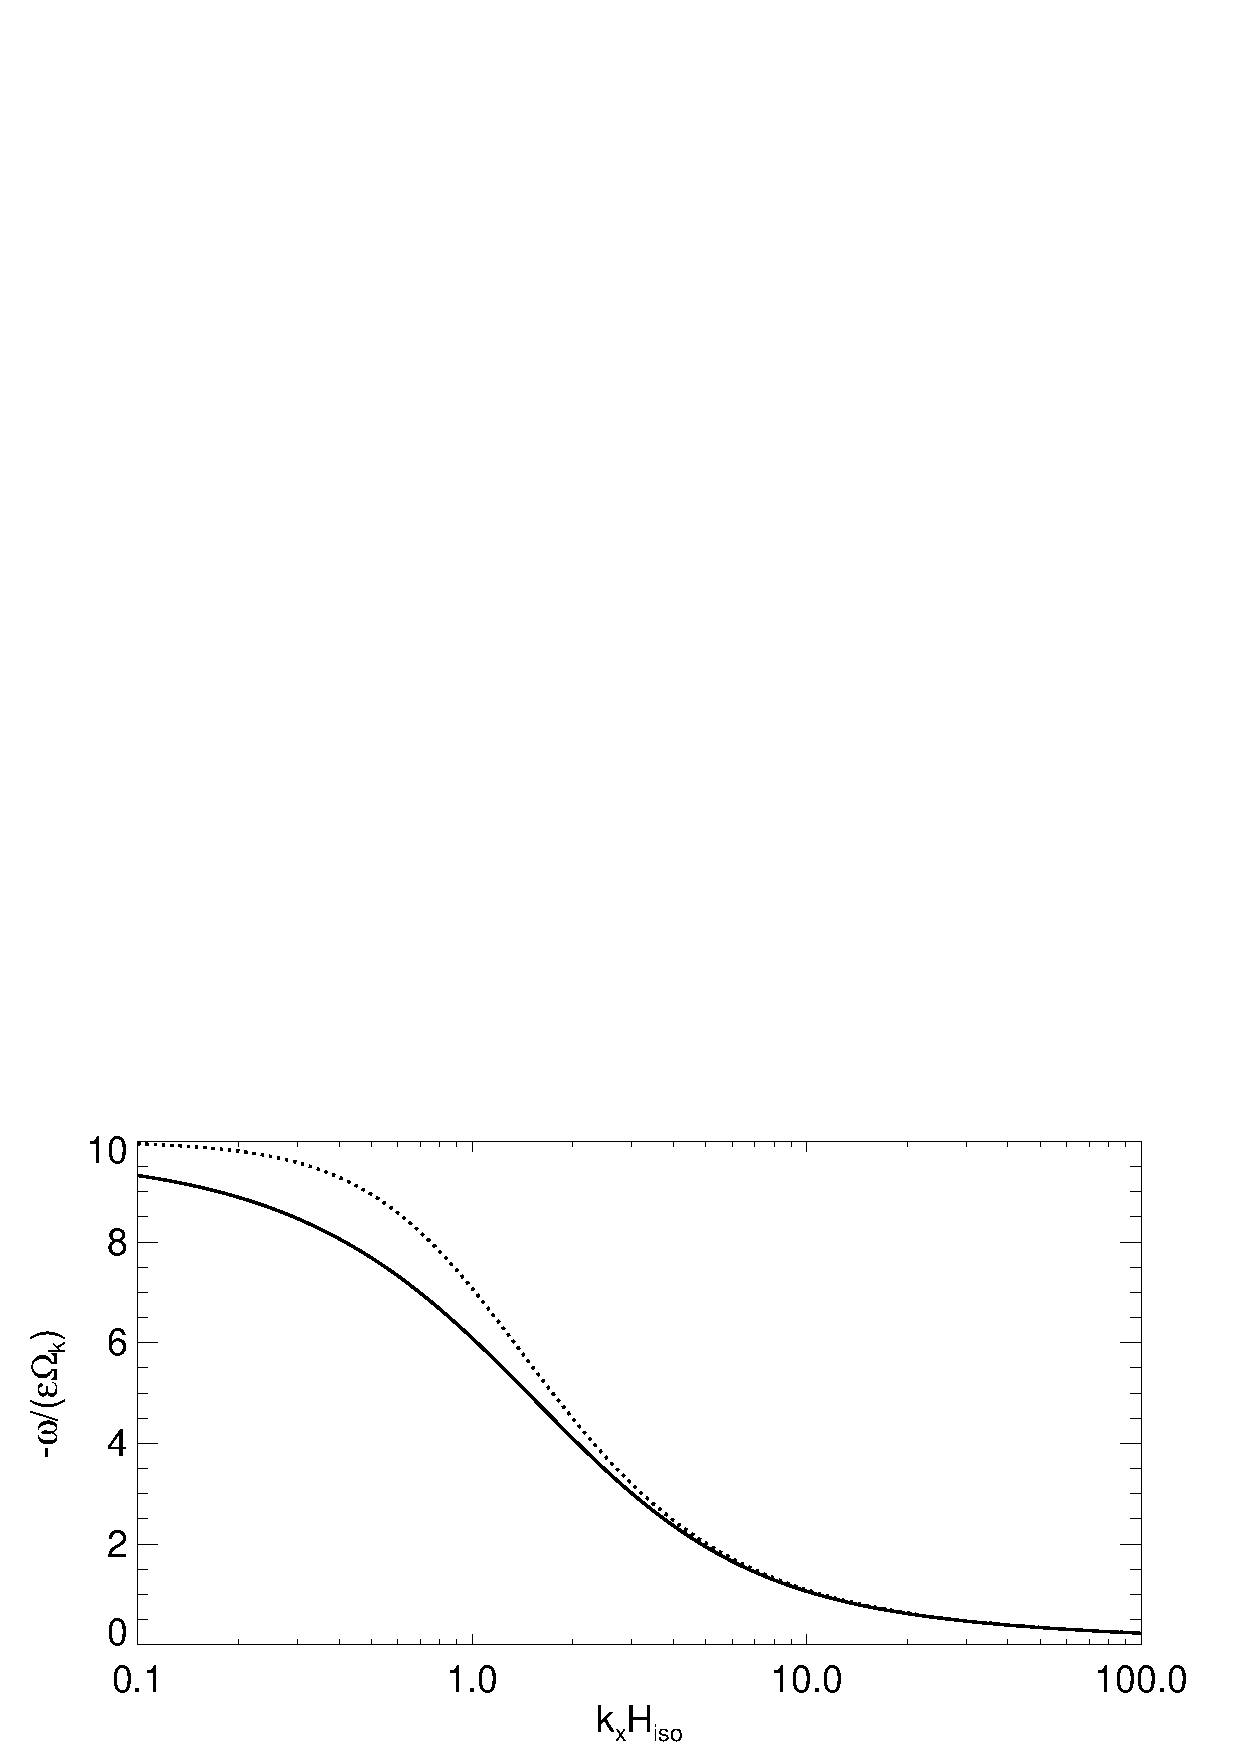
\includegraphics[width=\linewidth,clip=true,trim=0cm 0cm 0cm
%   1cm]{figures/compare_eigen_real_iso}
%   \caption{Growth rate (top) and real frequency (bottom) of the
%     fundamental VSI mode in the fiducial disk model with $\beta =
%     10^{-3}$. 
%     % a disk with $(\gamma,
%     % \Gamma)=(1.4,1.011)$, $(p,q, h)=(-1.5,-1,0.1)$ and
%     % $\beta=10^{-3}$. 
%     The solid (dotted) line is obtained numerically
%     (analytically).  
%     \label{iso_eigen_kx} 
%   }
% \end{figure}

% With rapid thermal relaxation, growth rates are expected to diminish
% for both $\khat\to 0$ and $\khat\to \infty$. This is because for
% $\khat\ll 1$ the radial wavelength is large, but such disturbances are 
% stabilized by by epicyclic motions ($|\omega|\sim
% \kappa$). Disturbances with $\khat\gg 1$ are radially localized, but  
% there is no energy change when fluid elements are perturbed at fixed
% cylindrical radius whilst conserving its angular momentum (applicable
% to axisymmetric perturbations).



\begin{figure}
  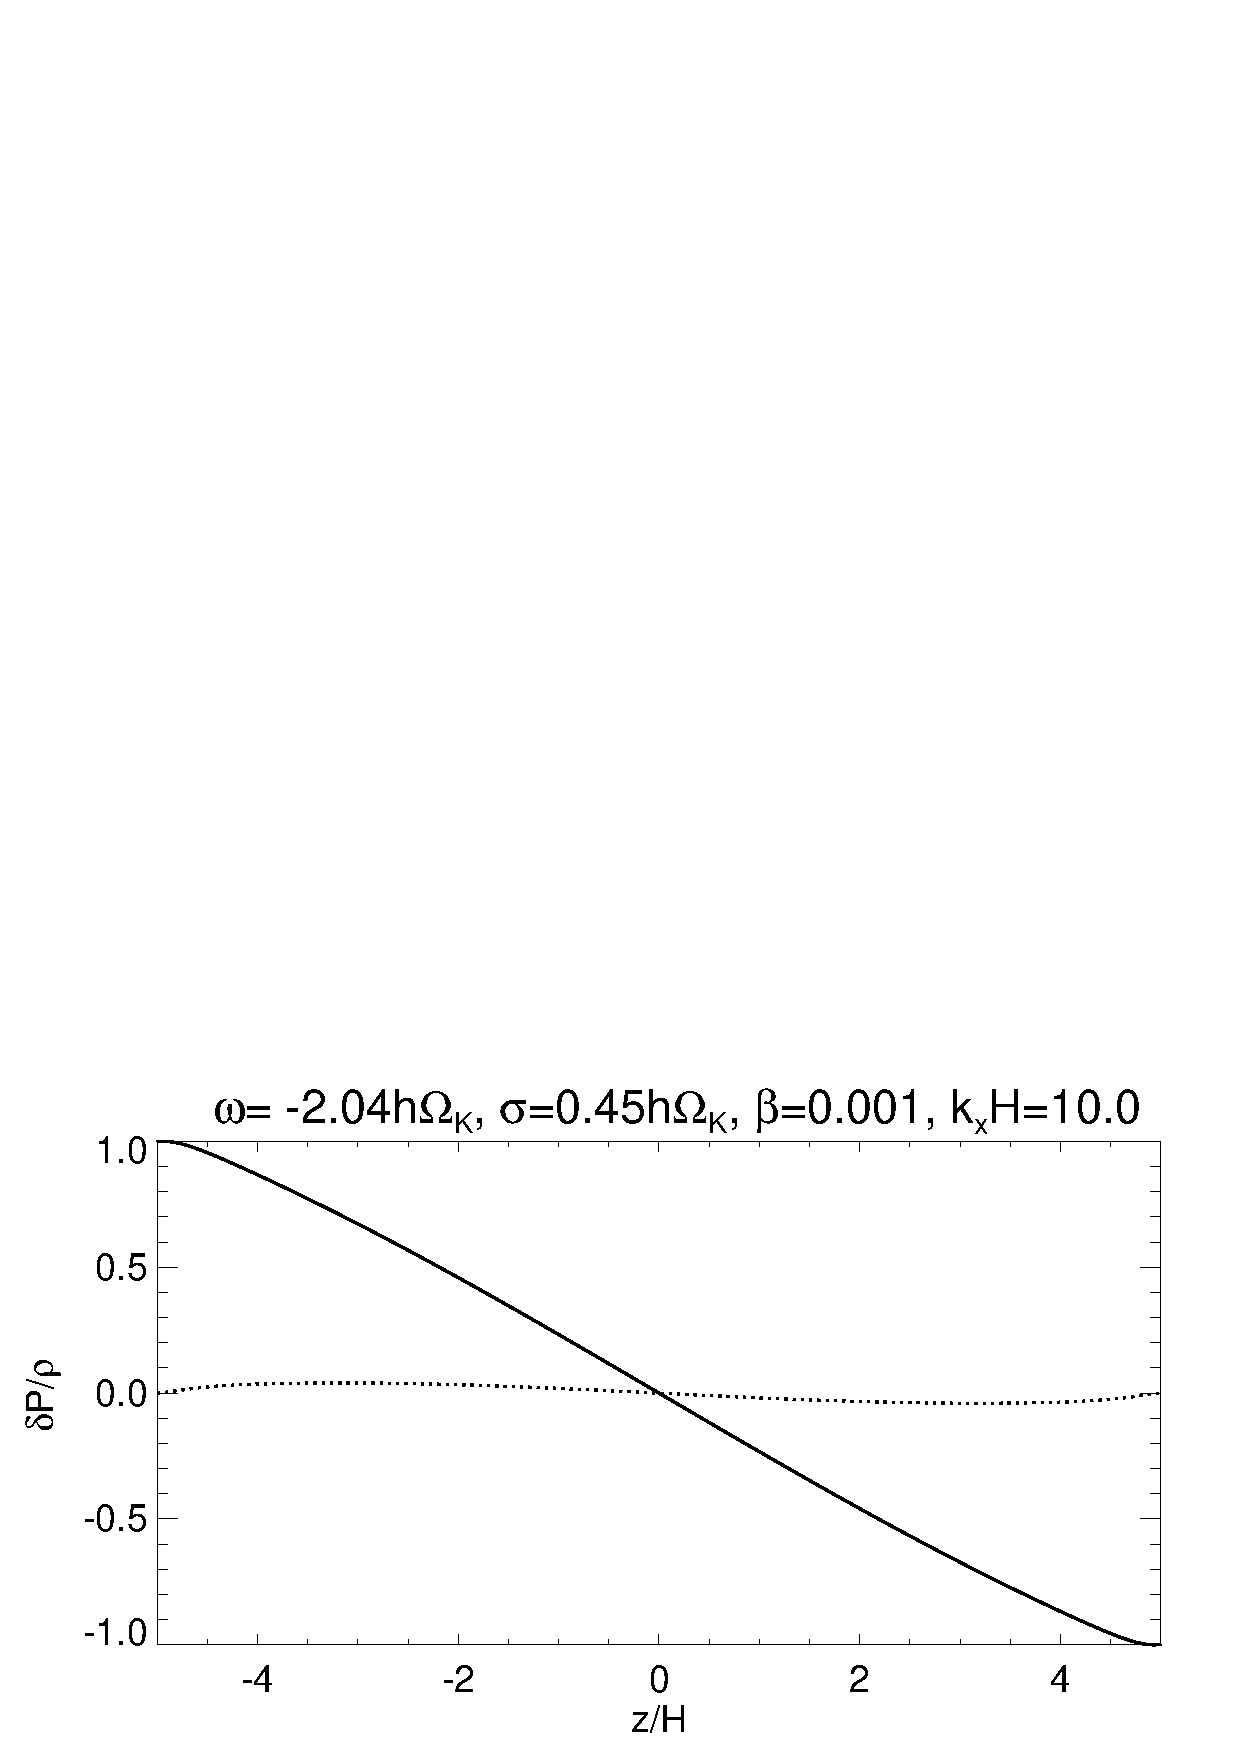
\includegraphics[width=\linewidth,clip=true,trim=0cm 1.75cm 0cm
  0cm]{figures/eigenvectorW_iso} 
  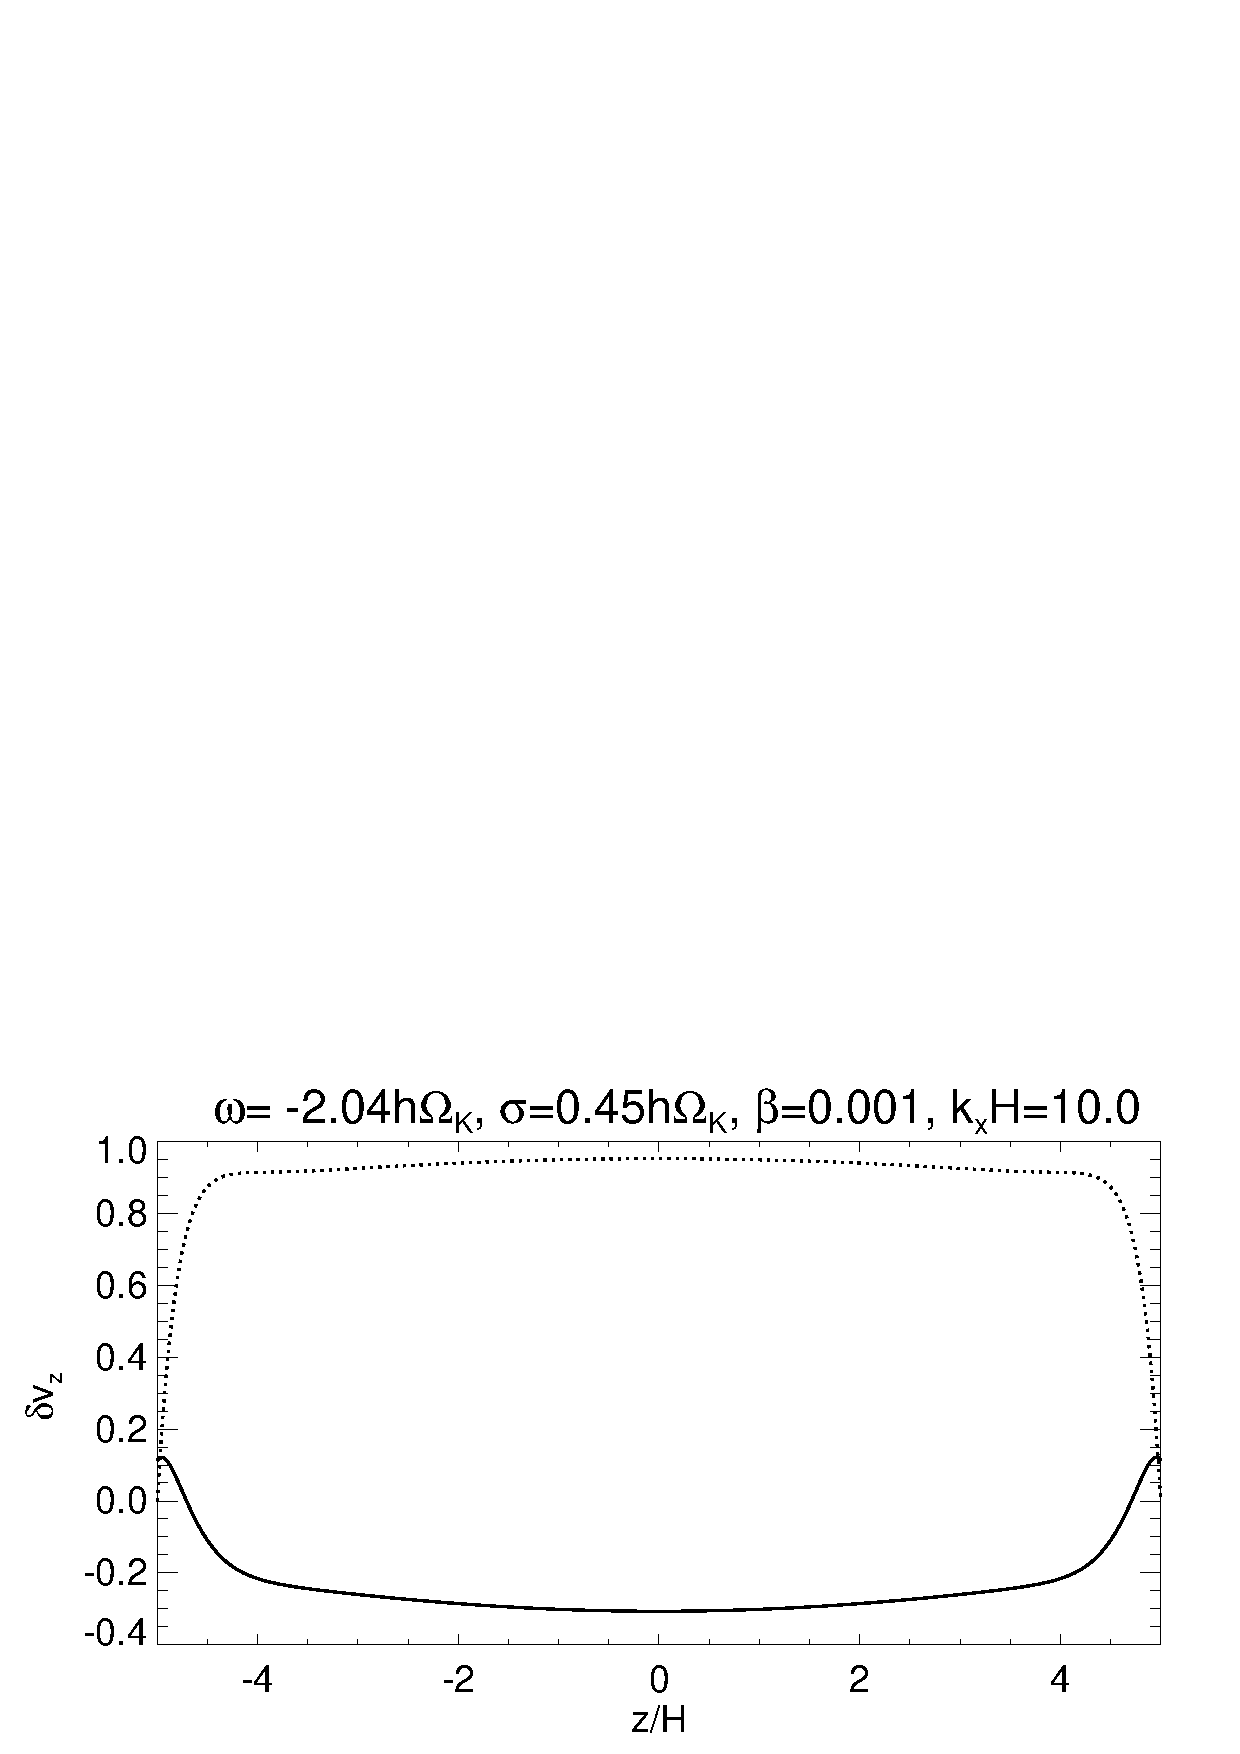
\includegraphics[width=\linewidth,clip=true,trim=0cm 0cm 0cm
  1cm]{figures/eigenvectorvz_iso}
  \caption{Pseudo-enthalpy perturbation $W$ (top) and vertical velocity
    perturbation $\delta v_z$ of the fundamental VSI with 
    $\khat=10$ in the fiducial disk with rapid thermal relaxation $\beta=10^{-3}$. The real  
    (imaginary) parts of $W$ and $\delta v_z$ are plotted as solid 
    (dotted) lines.  
    \label{lowfreq_eigenfunc}
  }
\end{figure}

\begin{figure}
%  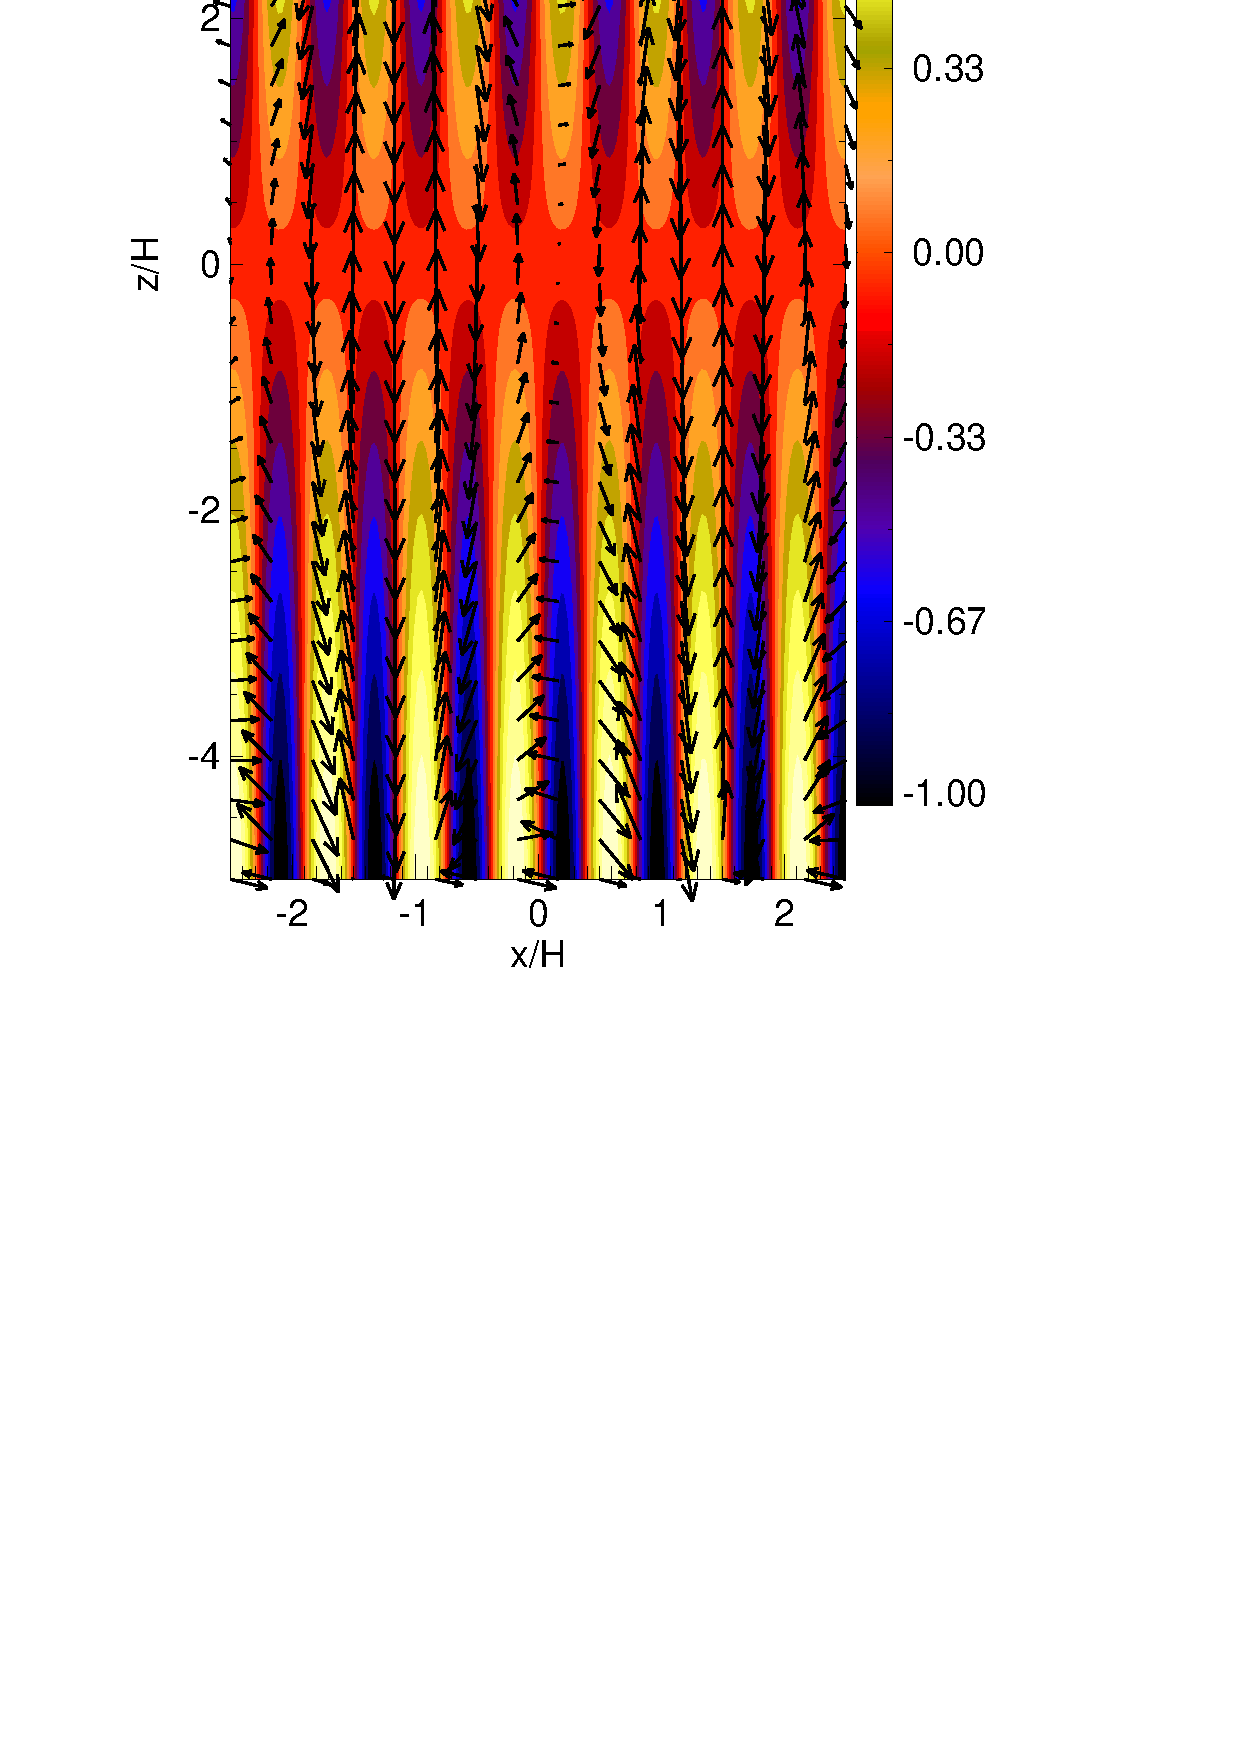
\includegraphics[scale=0.345,clip=true,trim=0cm 0cm 2.5cm
%  0cm]{figures/result2d_vel}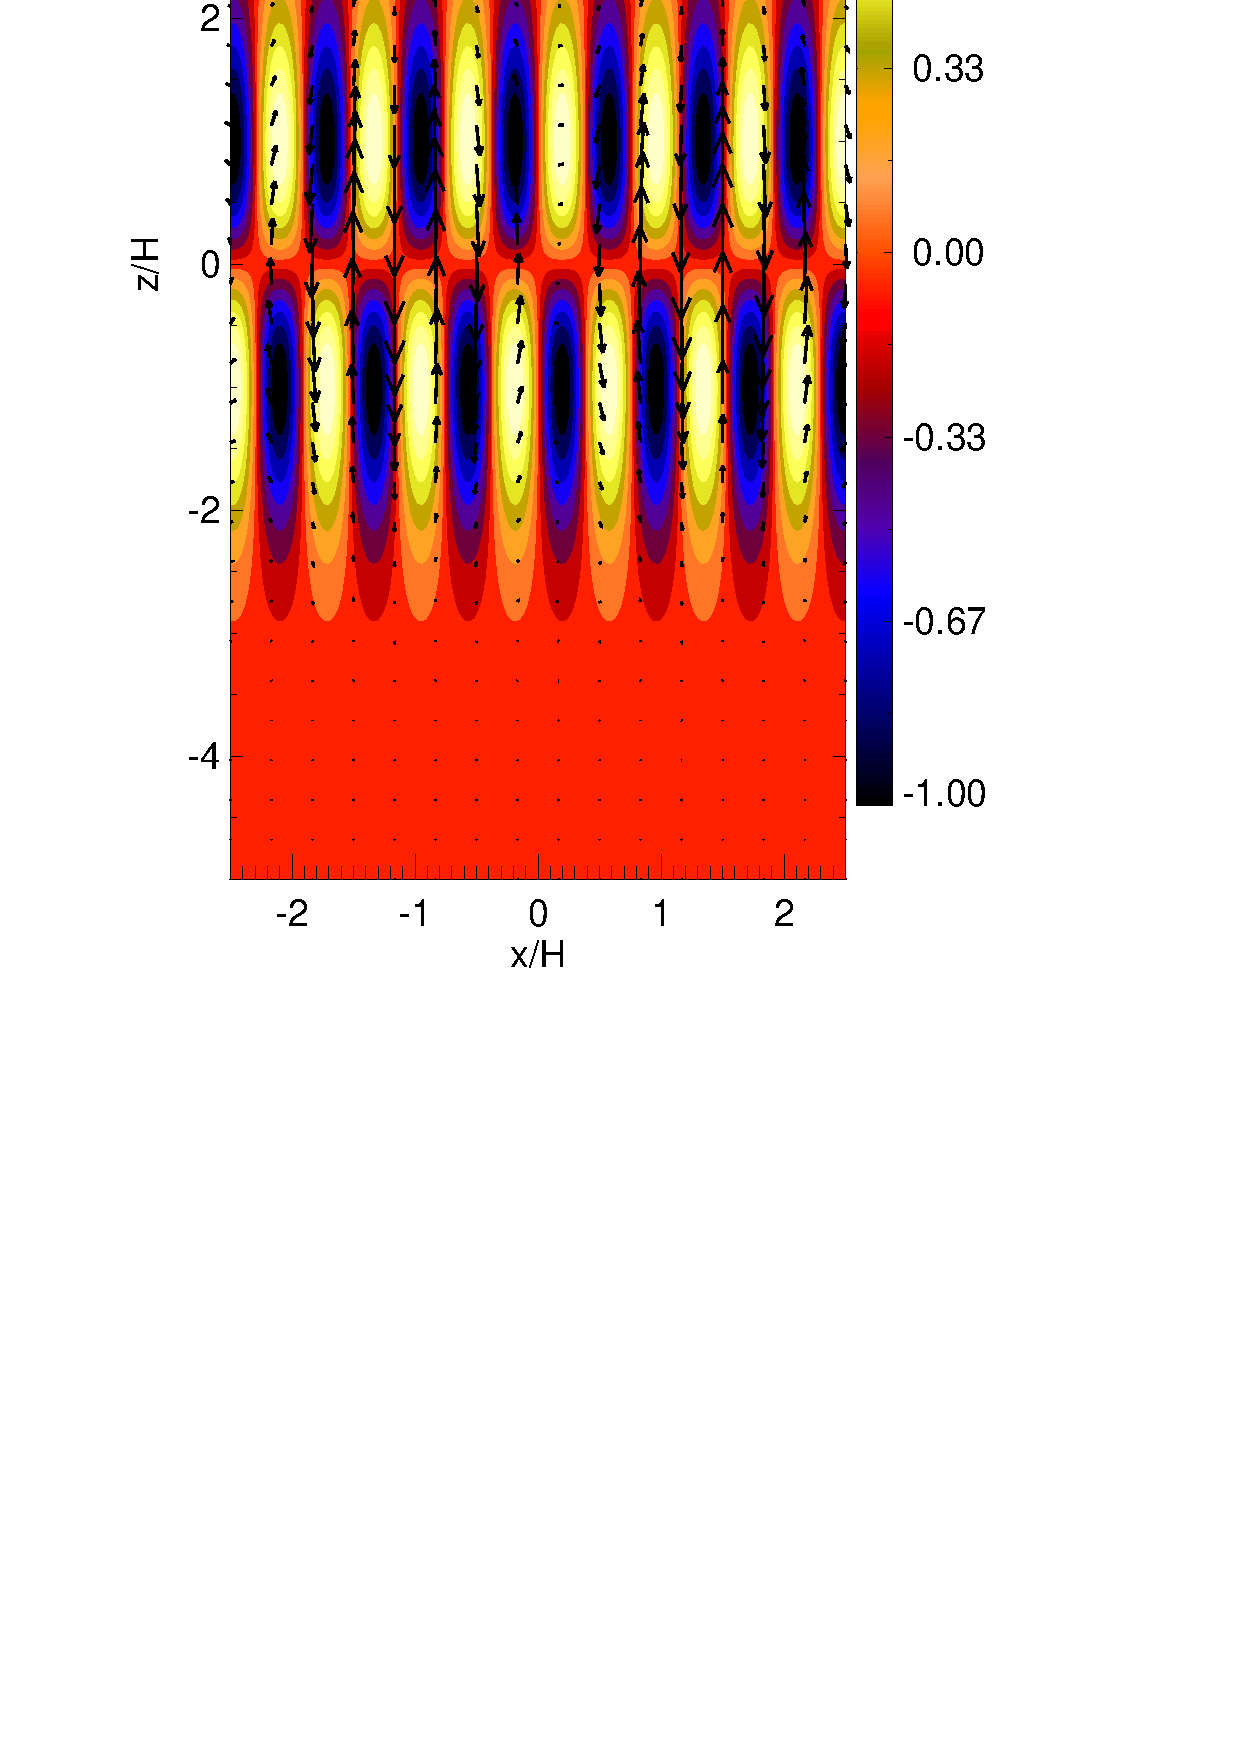
\includegraphics[scale=0.345,clip=true,trim=1.9cm 0cm 0cm
%  0cm]{figures/result2d_mom} 
  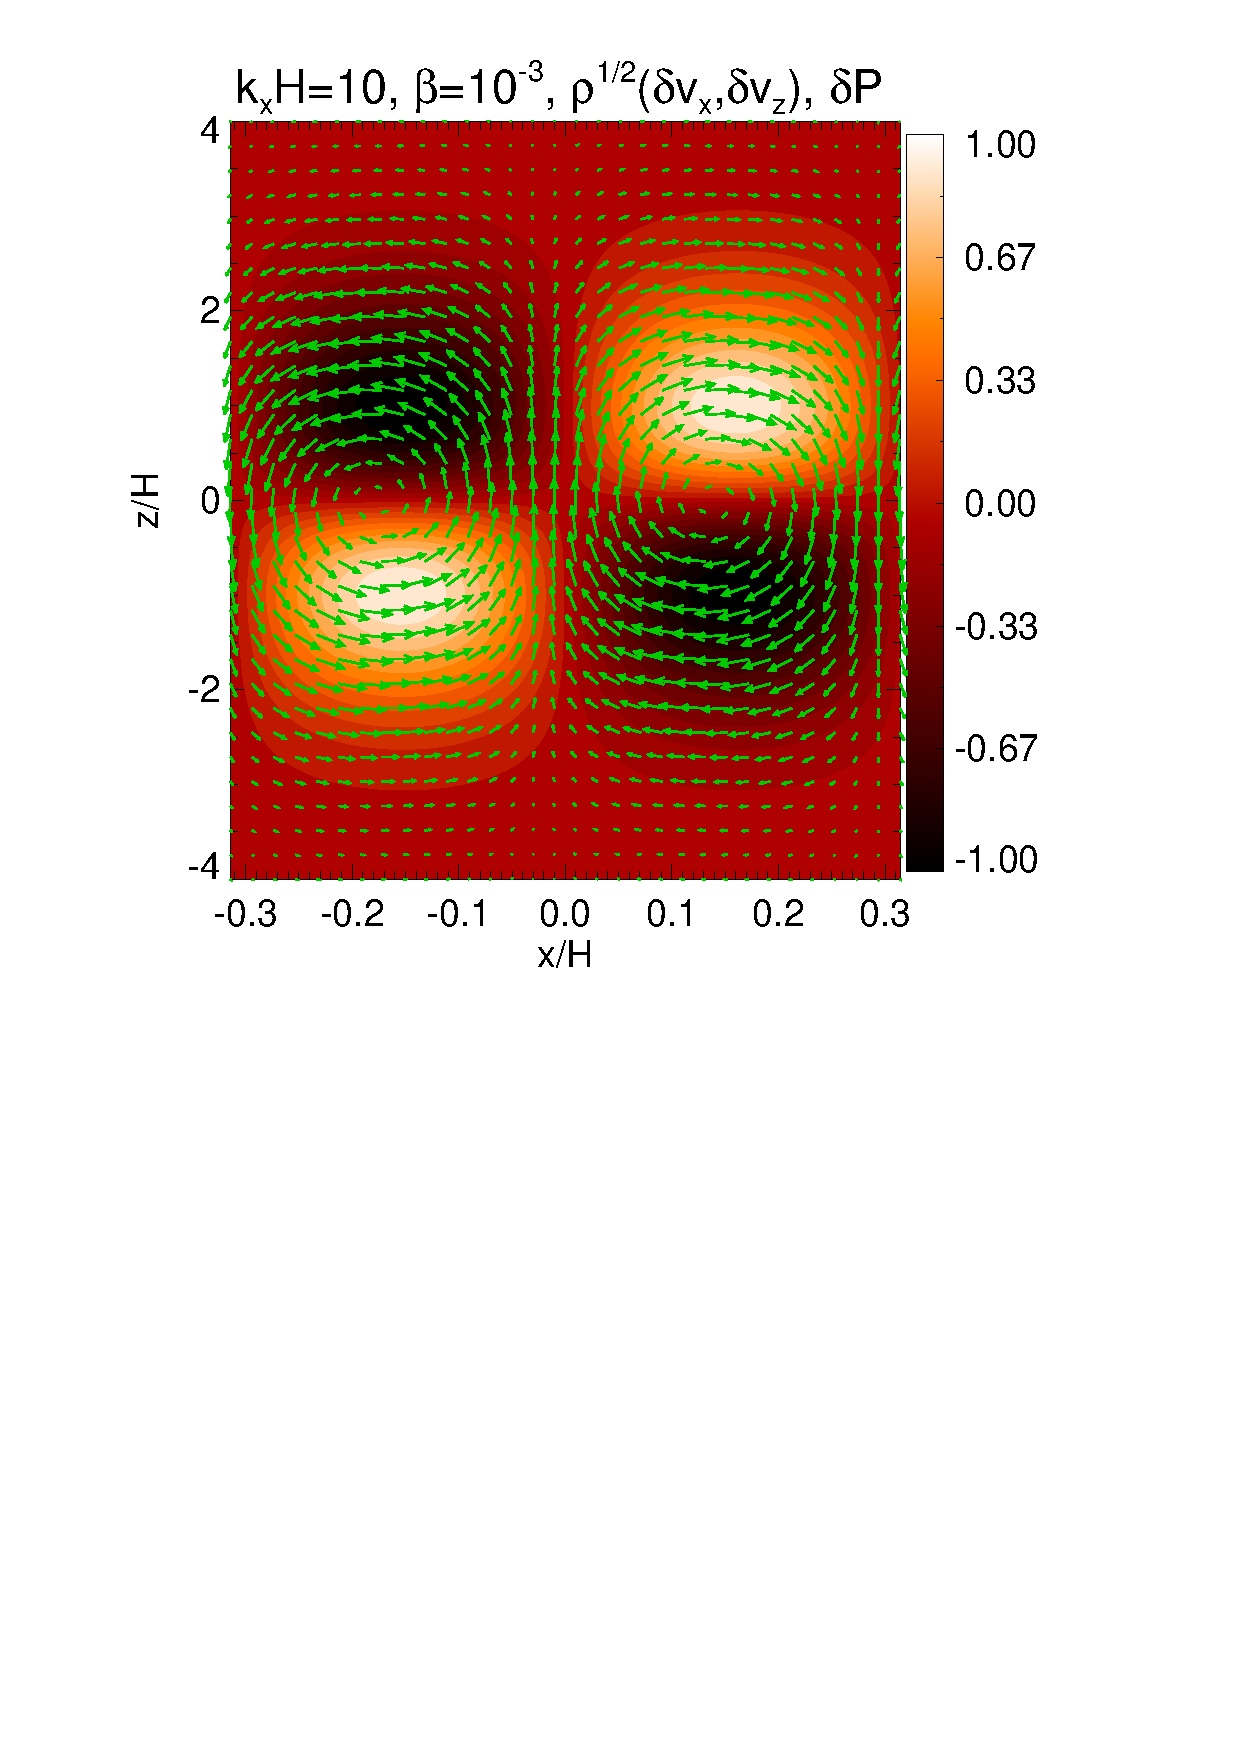
\includegraphics[width=\linewidth]{figures/result2d_iso}
  \caption{Visualization of the fundamental VSI mode in
    Fig. \ref{lowfreq_eigenfunc}. The color scale corresponds to the
    pressure perturbation $\delta P=\rho W$ scaled by its maximum value.
    Arrows show the flow, scaled as $\sqrt{\rho}(\delta
    v_x,\delta v_z)$. The horizontal axis has been stretched 
    for clarity.  
    \label{lowfreq_eigenfunc_2d}
  }
\end{figure}

\subsubsection{Case study: $\khat=10$}\label{k10}
Fig. \ref{compare_modes_iso_kx10} maps the growth rates $\sigma$ and
wave frequencies $\omega$ of unstable 
modes for $\khat=10$.  Each symbol 
corresponds to a different order mode, i.e.\ a different number of vertical node crossings.  Lower order modes
have smaller $|\omega|$ for fixed radial wavenumber, as expected for
inertial-gravity waves (see \S\ref{stable_novshear}).  

We compare our numerical results to the analytic dispersion relations for 
$\beta = 0$ and $10^{-3}$, from Eqs.\ \ref{simple_growth} and
\ref{relax_disp}, respectively.   The analytic models also have
discrete modes, which lie on the continuous curves that are plotted
for clarity in Fig. \ref{compare_modes_iso_kx10}.   While the analytic
models have many simplifications, they crucially lack an artificial
vertical surface (as they assume an infinite vertical domain).   

For our fiducial case (black dots), the lower order and lower
frequency modes closely follow the analytic prediction with growth
rates increasing with $|\omega|$. %, the magnitude of the frequency.
However, for $|\omega| \gtrsim 4 h \OmK$ the growth rate declines with
$|\omega|$.  This break from the analytic prediction is not due the
choice of boundary condition, as we demonstrate by considering rigid
boundaries (red plusses). 

Rather, the decline in growth rate for high order models is due to the
vertical box size, as seen by comparing the $\zmax/H = 3, 5$ and 7
cases in Fig. \ref{compare_modes_iso_kx10}. Increasing $\zmax$ give
better agreement with the analytic theory, which have $\zmax \to  
\infty$. Larger boxes include regions of larger vertical shear (see
Eqs. \ref{vshear_thin} and \ref{vertical_shear_ex}), which higher
order modes can tap to give larger growth rates. For the $\zmax = 7
H$ case, we begin to see another branch of modes with the highest
growth rates at $\omega \sim -6 h\OmK$. This branch contains the
`surface modes' described below.   

The need for vertically extended domains to capture the largest VSI
growth rates is problematic, especially for hydrodynamic simulations.
This  complication is mitigated by at least two factors.  First, we
show below that with slower cooling, the growth of higher order modes
is preferentially damped, consistent with the analytic analysis in
\S\ref{iso_vsi_beta_crit}.  Second, the fastest growing modes may not
dominate transport when they operate in very low density  surface
layers, i.e. at many $H$. Quantifying which modes will contribute
most to non-linear transport is an important issue, but beyond the
scope of this work. 


%comment: the following reads like a figure caption, not a description of results.
%Black dots correspond to our fiducial setup.  
%We also plot results obtained with different 
%vertical boundary conditions: rigid boundary and $\zmax=5H$ (red
%crosses),  free surface and $\zmax = 3H$ (blue triangles), free surface
%and $\zmax=7H$ (green crosses). 

%The modes shown in Fig. \ref{compare_modes_iso_kx10} are `body modes'
%and are inertial waves destabilized by vertical shear
%\citepalias{barker15}. (The exception being the fastest growing
%mode for $\zmax=7H$ which is a surface mode --- see the discussion
%below.)  The `fundamental corrugation mode', marked by `f',
%corresponds to the eigenvalue with the smallest $|\upsilon|$. The
%fundamental mode is robust  
%against vertical boundary conditions as it appears at the same
%position in Fig. \ref{compare_modes_iso_kx10} for all cases. Higher  
%order modes, corresponding to increasing $|\omega|$, increasingly
%deviates from the analytic line due to the imposed boundaries, 
%unless $\zmax$ is increased. 

Fig. \ref{lowfreq_eigenfunc} shows 
eigenfunctions $W = \delta P/\rho$ and $\delta   v_z$ for the lowest order fundamental mode.  
Fig. \ref{lowfreq_eigenfunc_2d} maps the pressure perturbation and meridional flow,
scaled by $\sqrt{\rho}$ to reflect the contribution to kinetic
energy. Notice the stretched $x$ axis. Radial velocities are in fact typically much 
smaller than vertical velocities, as expected for a vertically
elongated, anelastic mode \citepalias{nelson13}. Most of the kinetic
energy is contained within $\sim 2H$ of the midplane due to the
density stratification.  

\begin{figure}
  \includegraphics[width=\linewidth]{figures/compare_modes_iso_kx30_analytic.ps}
  \caption{Same as Fig. \ref{compare_modes_iso_kx10} but for
    $\khat=30$. Examples of surface modes are 
    marked by `s'. \label{compare_modes_iso_kx30}
  }
\end{figure}


\begin{figure}
  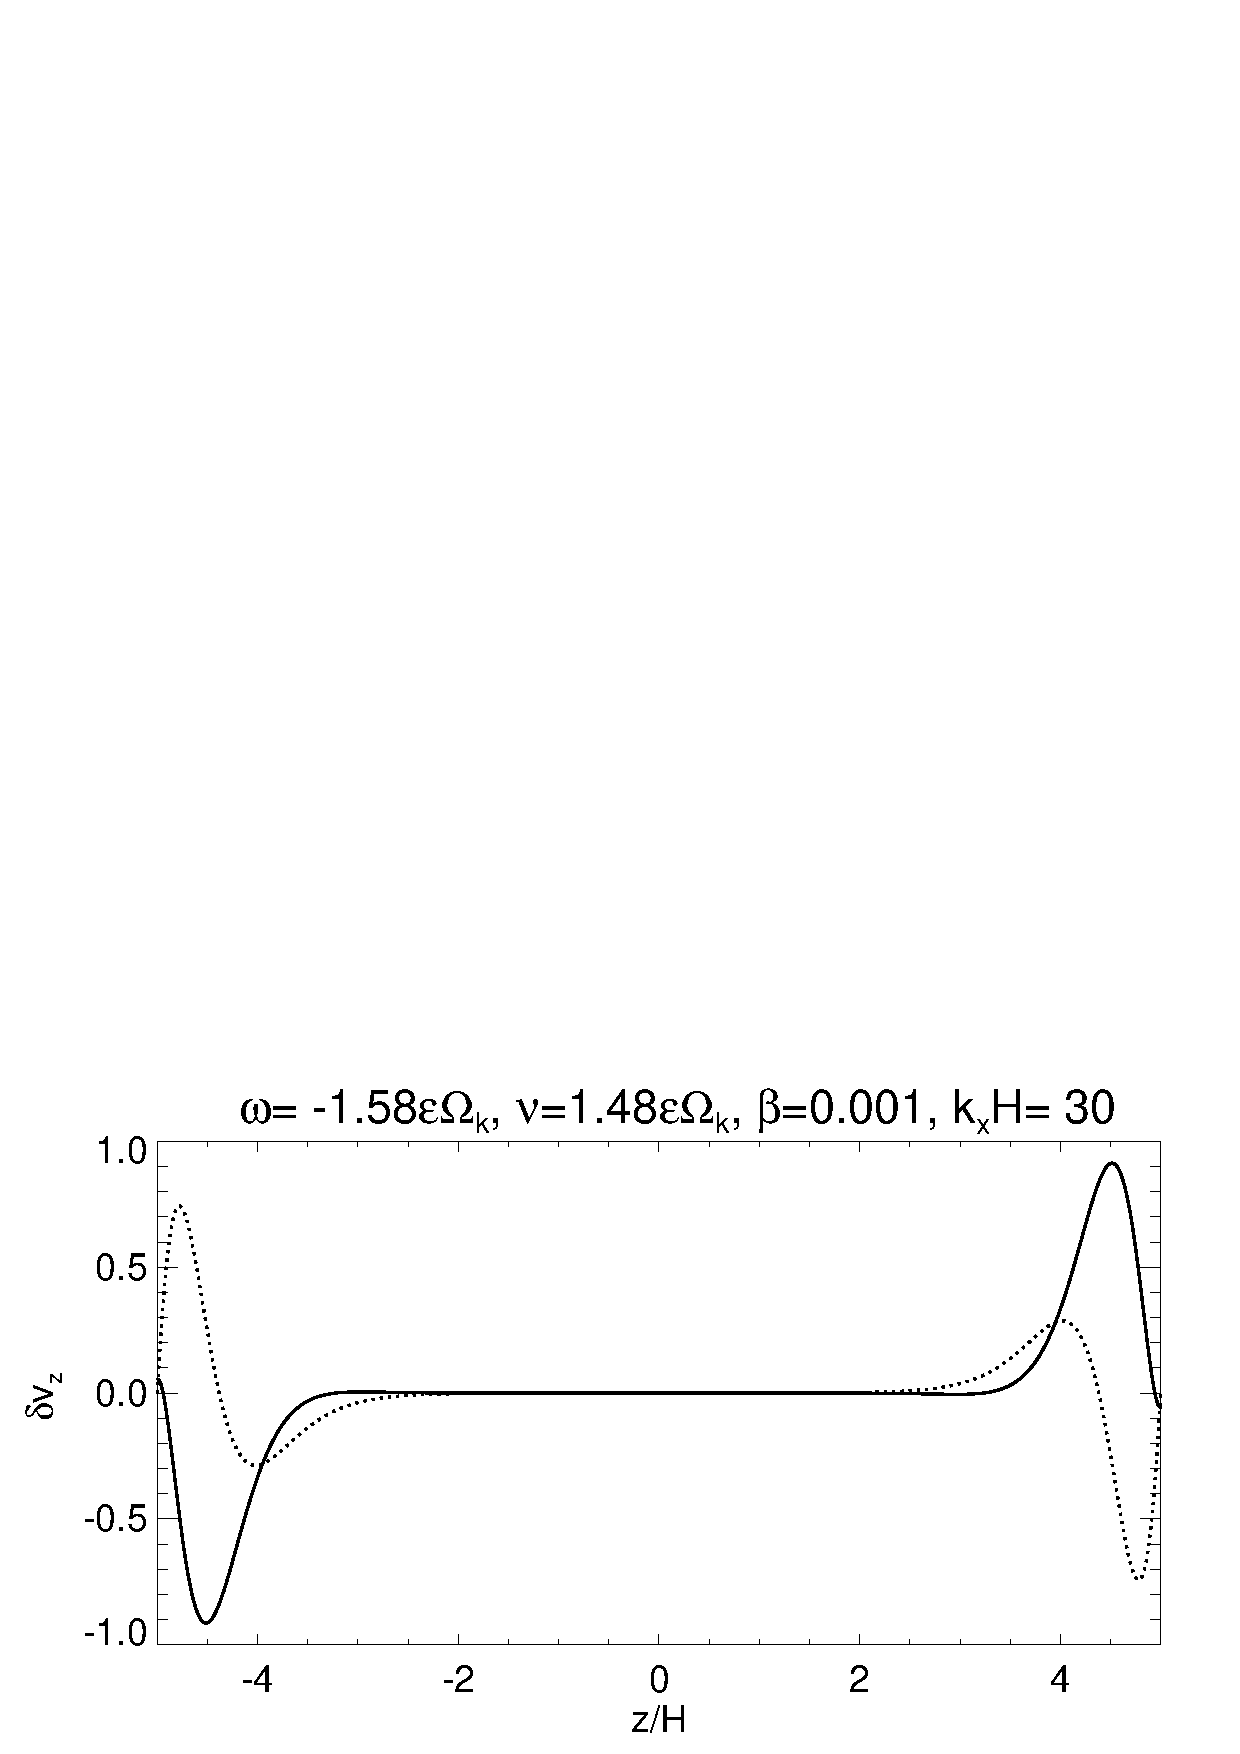
\includegraphics[width=\linewidth,clip=true,trim=0cm 0cm 0cm
  0cm]{figures/eigenvectorvz_iso_surf}
  \caption{Example of a `surface mode' in the fiducial disk model.
    \label{lowfreq_eigenfunc_surf}
  }
\end{figure}

\subsubsection{Surface modes of the VSI}\label{surf_comment} 
The surface modes mentioned above are more prominent for larger
wavenumbers. Fig. \ref{compare_modes_iso_kx30} maps the $\khat = 30$
eigenvalues, with the surface modes labelled.  The surface modes
strongly depend on the location of the imposed vertical boundary, and
disagree with the analytic models, which lack an imposed surface. We
thus discount the physical significance of surface modes for our
model, as we explain further below.  

Surface modes are a well known feature of the VSI in finite vertical
domains \citepalias{nelson13, mcnally14}. \citetalias{barker15} show
that surface modes arise whether the surface is artificial (as for our
imposed $\zmax$) or natural (for disk models with a zero density surface).
Physical surface modes are in principle possible; BL15 mention
surfaces between a disk's interior and corona.  In models where the
surface is imposed, like ours, surface modes are a numerical
artifact. 

The possibility of artificial surface modes seeding growth in
numerical simulations of the VSI  merits further study. Indeed
\citetalias{nelson13} find that the initial growth of perturbations
primarily occurs near the vertical boundaries. 
The motion in surface modes is indeed concentrated near the surface,
as shown in Fig. \ref{lowfreq_eigenfunc_surf}.   
Thus even if surface modes were physical, their contribution to
transport might (by themselves) be weak,  following the arguments in 
\S\ref{k10}.  Moreover surface modes, like all modes with large
wavenumbers, are more prone to viscous damping, as discussed in
\S\ref{caveats_visc}. 

While the relatively large growth rates of surface modes is
tantalizing, we dismiss them in disk models that lack a physical
surface.  


%...
%This a class of unstable modes associated with vertical shear near the
%disk boundaries. They are absent in our  
%analysis because there we assumed a disk with infinite 
%vertical extent, since the vertically isothermal disk has no
%surface. However, surface modes can occur in the present calculations 
%because there is an imposed vertical boundary.   
%
%We illustrate surface modes in Fig. \ref{compare_modes_iso_kx30} 
%which show unstable modes with $\khat=30$. Surface 
%modes lie almost parallel to the vertical axis 
%in such diagrams. They are readily identified for  $\zmax\geq 5H$ and
%are marked by `s'.  Fig. \ref{lowfreq_eigenfunc_surf} shows an example
%of a surface mode. We typically find an increasing
%number of surface modes with increasing $\zmax$ and/or $\khat$. 
%%consistent with \cite{barker15}. 
% 
%As explained by \citetalias{barker15}, while surface modes have a physical
%origin, their occurence in the vertically isothermal disk is due to
%imposing a finite vertical domain size. This has important
%implications when interpreting results obtained from the vertically
%isothermal disk model. For example, seeking the most unstable mode may
%result in a surface mode, but its growth rate would depend on
%$\zmax$. We return to this issue later.     

%Thus, the
%vertically isothermal disk is not useful for studying surface modes. 
%Thus, seeking the most unstable mode in a vertically isothermal disk
%may not yield robust results because this 



\begin{figure}
  \includegraphics[width=\linewidth,clip=true,trim=0cm 1.75cm 0cm
  0cm]{figures/compare_modes_cool_kx10_z3_analytic.ps} 
  \includegraphics[width=\linewidth,clip=true,trim=0cm 1.75cm 0cm
  0cm]{figures/compare_modes_cool_kx10_z5_analytic.ps}
  \includegraphics[width=\linewidth]{figures/compare_modes_cool_kx10_z7_analytic.ps}
  \caption{Unstable modes with $\khat=10$ and thermal
    relaxation timescales $\beta=0.01$ (black dots), $\beta=0.03$ (red
    crosses), $\beta=0.05$ (blue triangles) and $\beta=0.1$ (green 
    crosses); for different vertical domain sizes $\zmax=3H$ (top),
    $\zmax=5H$ (middle, the fiducial setup) and $\zmax=7H$
    (bottom). Lines are computed from
    Eq. \ref{relax_disp} for  $M=0$ (solid, fundamental mode) and
    $M=1,\,2,\,3$ (dotted, dashed, dash-dot, respectively). Along each
    line, $\beta$ increases continuously from $0.01$ to $0.1$ from top
    to bottom, and squares mark corresponding $\beta$ values with
    numerical results. 
    \label{compare_modes_cool_kx10} 
  }
\end{figure}

\subsection{Slower thermal relaxation}\label{therm_relax_eff}
We now consider the effect of longer cooling timescales by gradually
increasing  
$\beta$. We expect VSI growth for  $\beta < \beta_\mathrm{crit} =
0.125$.  We also expect that higher order modes will damp at even
lower $\beta$ values, as argued in \S\ref{iso_vsi_beta_crit}. 

Fig. \ref{compare_modes_cool_kx10} largely confirms these expectations
by plotting eigenvalues for $\khat=10$  
and $\beta$ from $0.01$ to  $0.1$.  
The analytic results from Eq. \ref{relax_disp} are now plotted as
different curves for each mode order $M$, with $\beta$ varying along
each curve. We see the standard increase in frequency, $|\omega|$,
with mode order. 

As expected, the higher order modes are preferentially damped.  For
$\beta \geq 0.03$ the fundamental ($M = 0$) mode is the fastest
growing. For $\beta = 0.1$, only the $M = 0$ mode grows. This growth
is slow since $\beta$ is near $\beta_\mathrm{crit}$. 

Fig. \ref{compare_modes_cool_kx10} also shows how cooling times affect
the dependence on $\zmax$, the size of the vertical domain.   For all
cooling times, the fundamental mode depends only weakly on $\zmax$,
and there is good agreement with analytic values.  This convergence is
reassuring given the importance of the fundamental mode at longer
cooling times.  For higher order modes and short cooling times,
however, the eigenvalues vary strongly with $\zmax$.  The disagreement
with analytic theory is strongest for the smallest domain, with $\zmax
= 3 H$.  For $\beta \geq 0.03$, the $\zmax/H = 5, 7$ and the analytic
results are well converged (aided by the fact that only $M < 5$ modes
grow). 


%We find the number of unstable modes decrease with increasing
%$\beta$. Consider the fiducial setup with $\zmax=5H$ 
%(middle panel). The fundamental mode ($M=0$) is not the most unstable for   
%$\beta=0.01$ as higher order modes have larger
%growth rates. As noted above, these higher order modes are affected by
%$\zmax$, e.g. there is a significant mismatch between numerical and 
%analytical results for $M\geq1$ when $\zmax=3H$ (upper panel). 
%
%However, the fundamental mode becomes dominant for $\beta \geq 
%0.03$. Higher order modes, which would be dominant at small $\beta$, 
%are more effectively stabilized with increasing $\beta$. For 
%$\beta=0.1$, which is close to the critical thermal timescale
%$\beta_\mathrm{crit} (=0.125$ for the fiducial disk
%parameters), we only find the fundamental mode. This is consistent with
%the discussion in \S\ref{iso_vsi_beta_crit}.    

\begin{figure}
  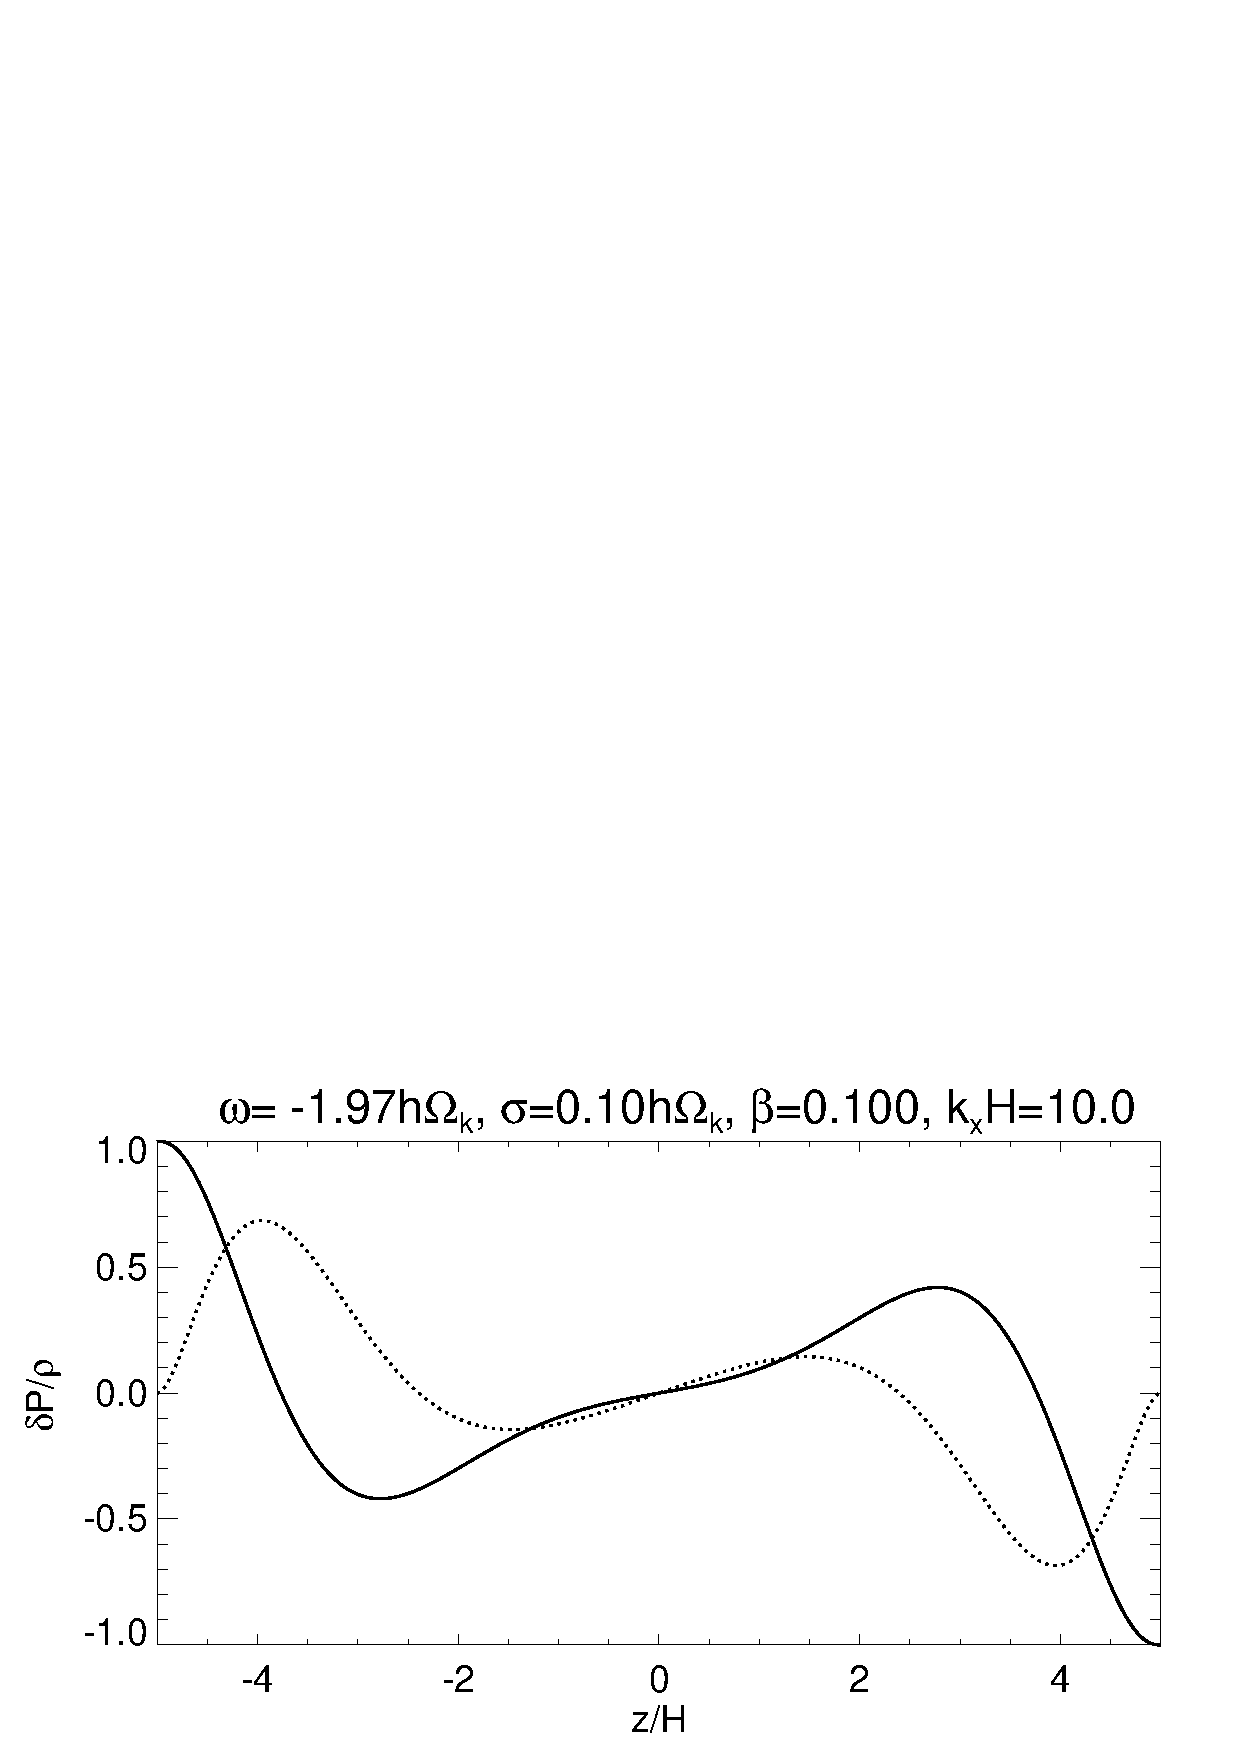
\includegraphics[width=\linewidth,clip=true,trim=0cm 1.75cm 0cm
  0cm]{figures/eigenvectorW_beta0d1} 
  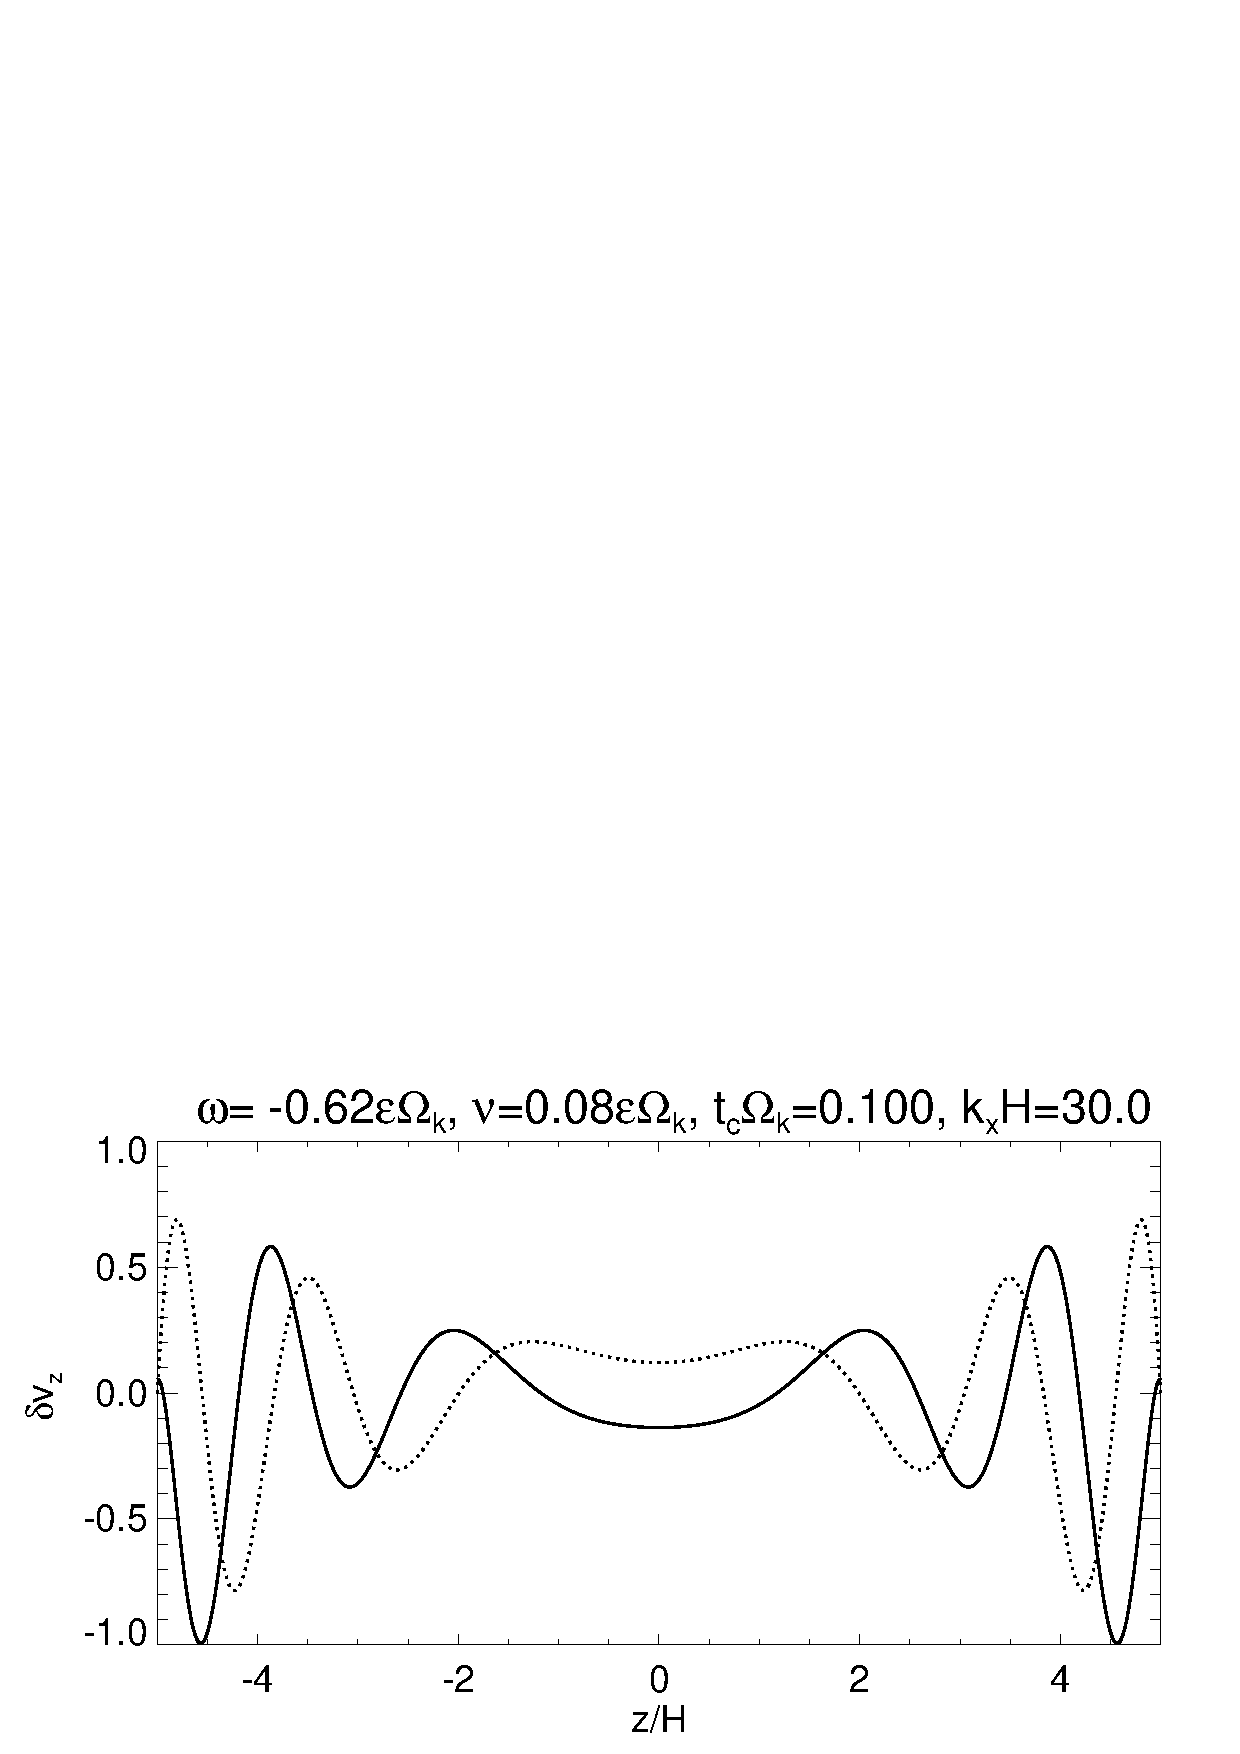
\includegraphics[width=\linewidth,clip=true,trim=0cm 0cm 0cm
  1cm]{figures/eigenvectorvz_beta0d1}
  \caption{Same as Fig. \ref{lowfreq_eigenfunc} but with a
    thermal relaxation timescale $\beta=0.1$. 
    \label{lowfreq_eigenfunc_cool}
  }
\end{figure}

\begin{figure}
  % 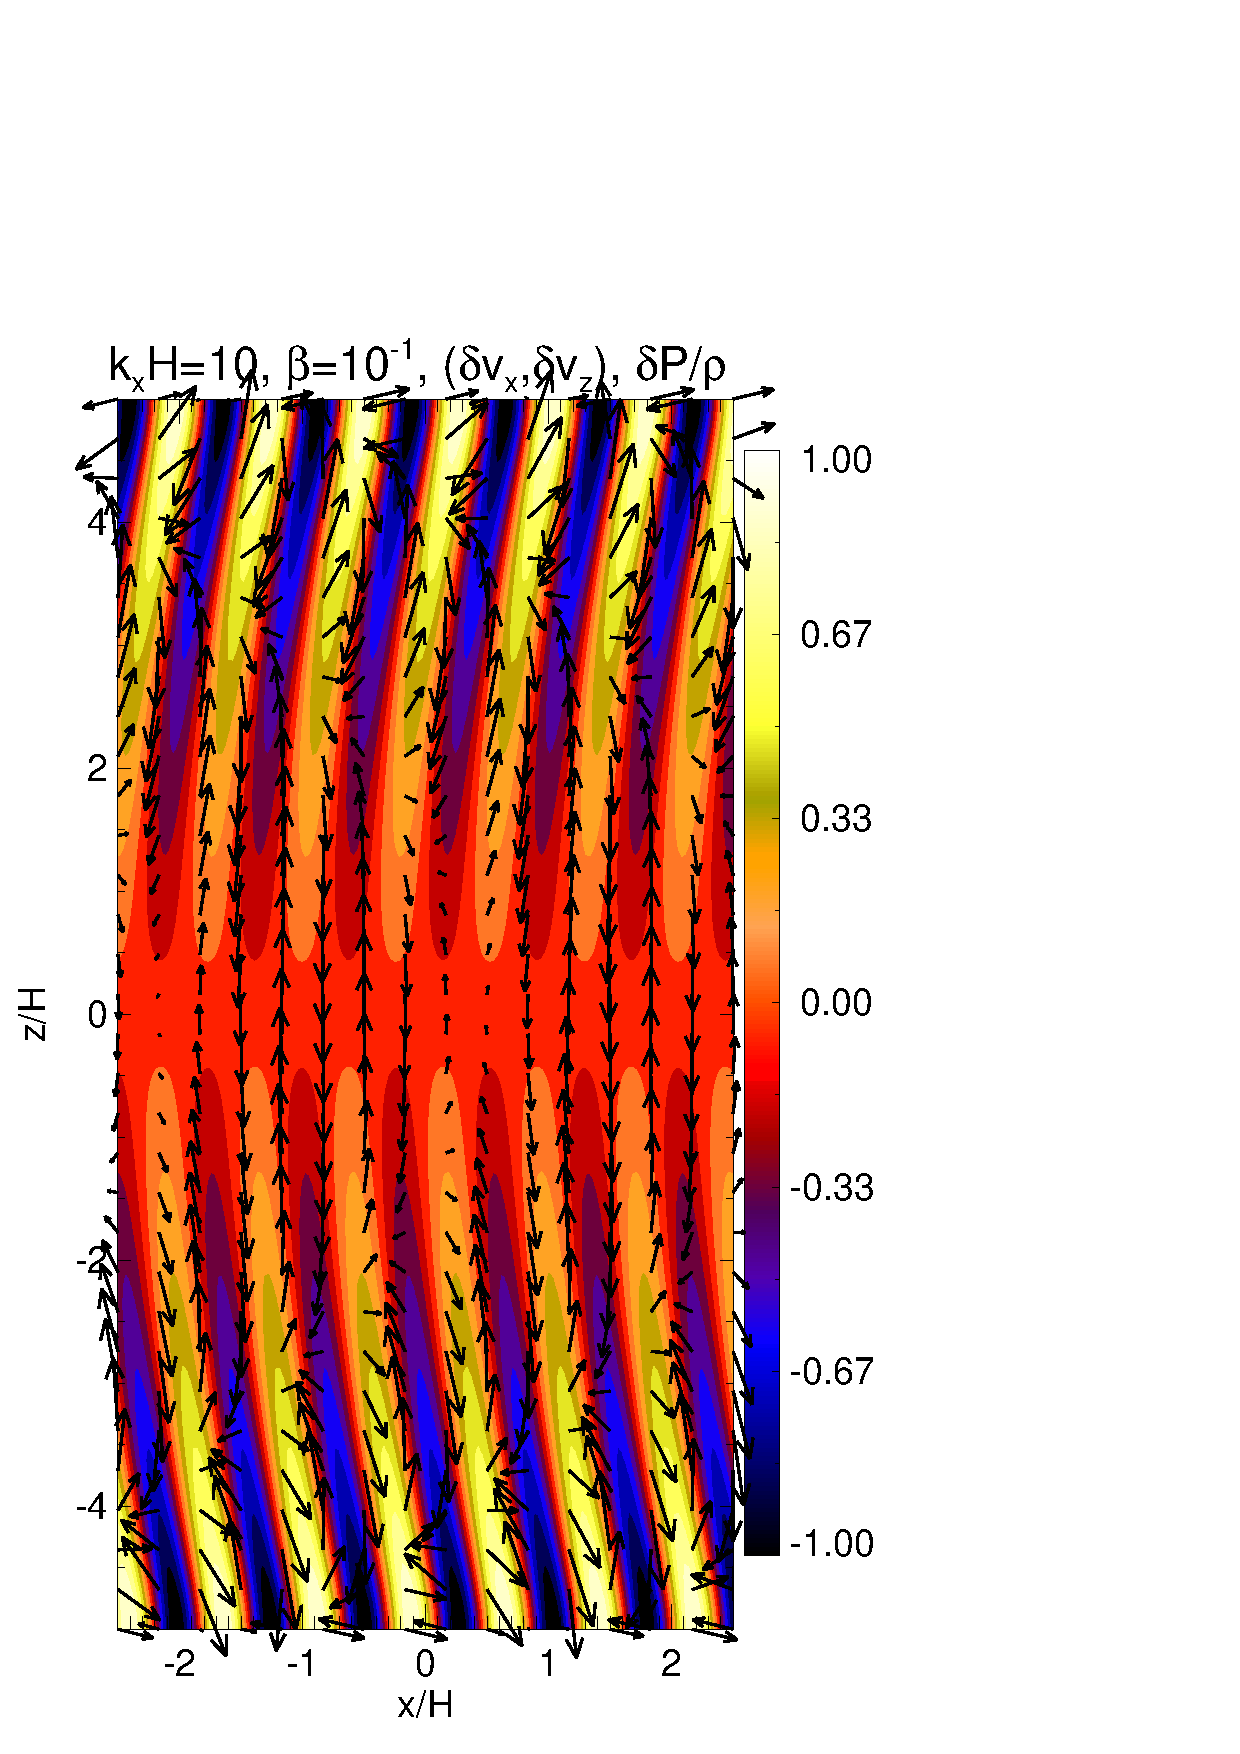
\includegraphics[scale=0.345,clip=true,trim=0cm 0cm 2.5cm
  % 0cm]{figures/result2d_vel_cool}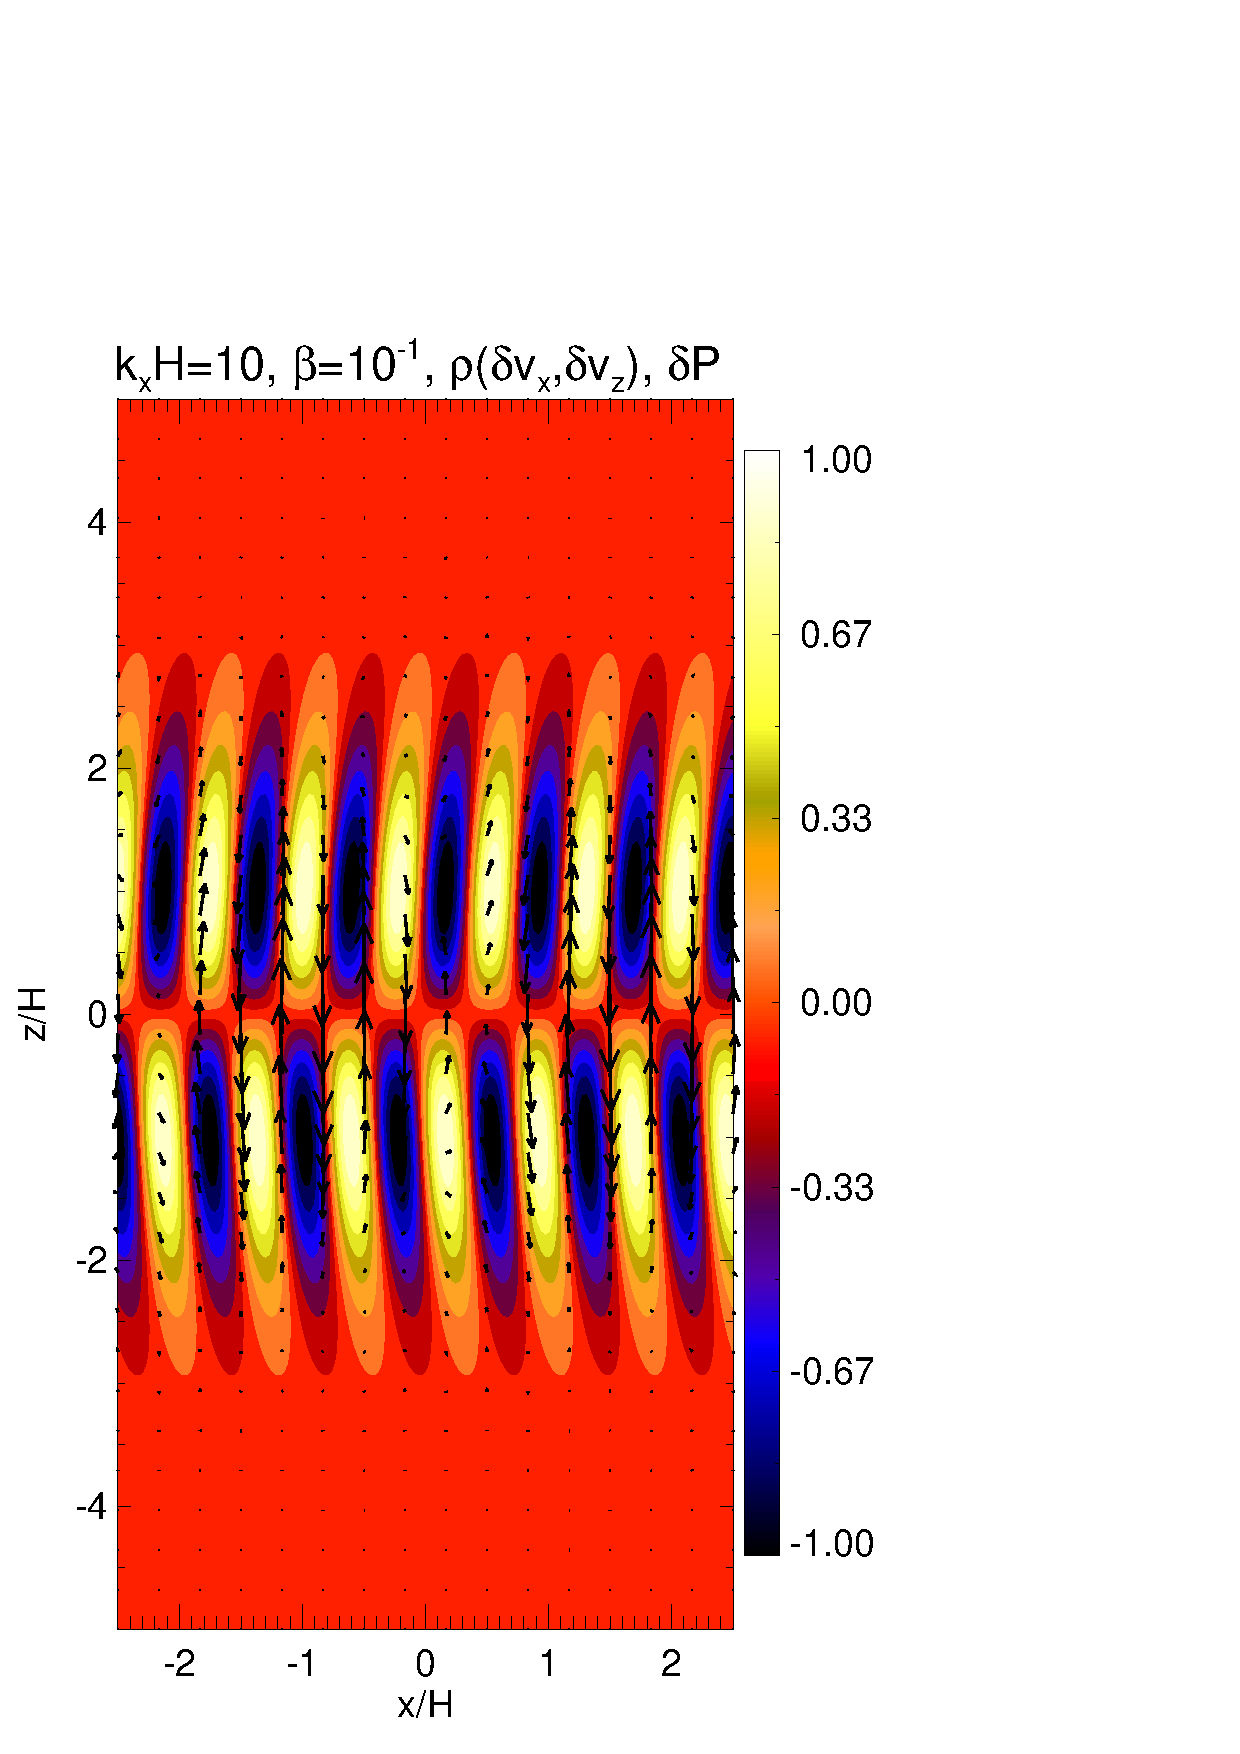
\includegraphics[scale=0.345,clip=true,trim=1.9cm 0cm 0cm
  % 0cm]{figures/result2d_mom_cool} 
  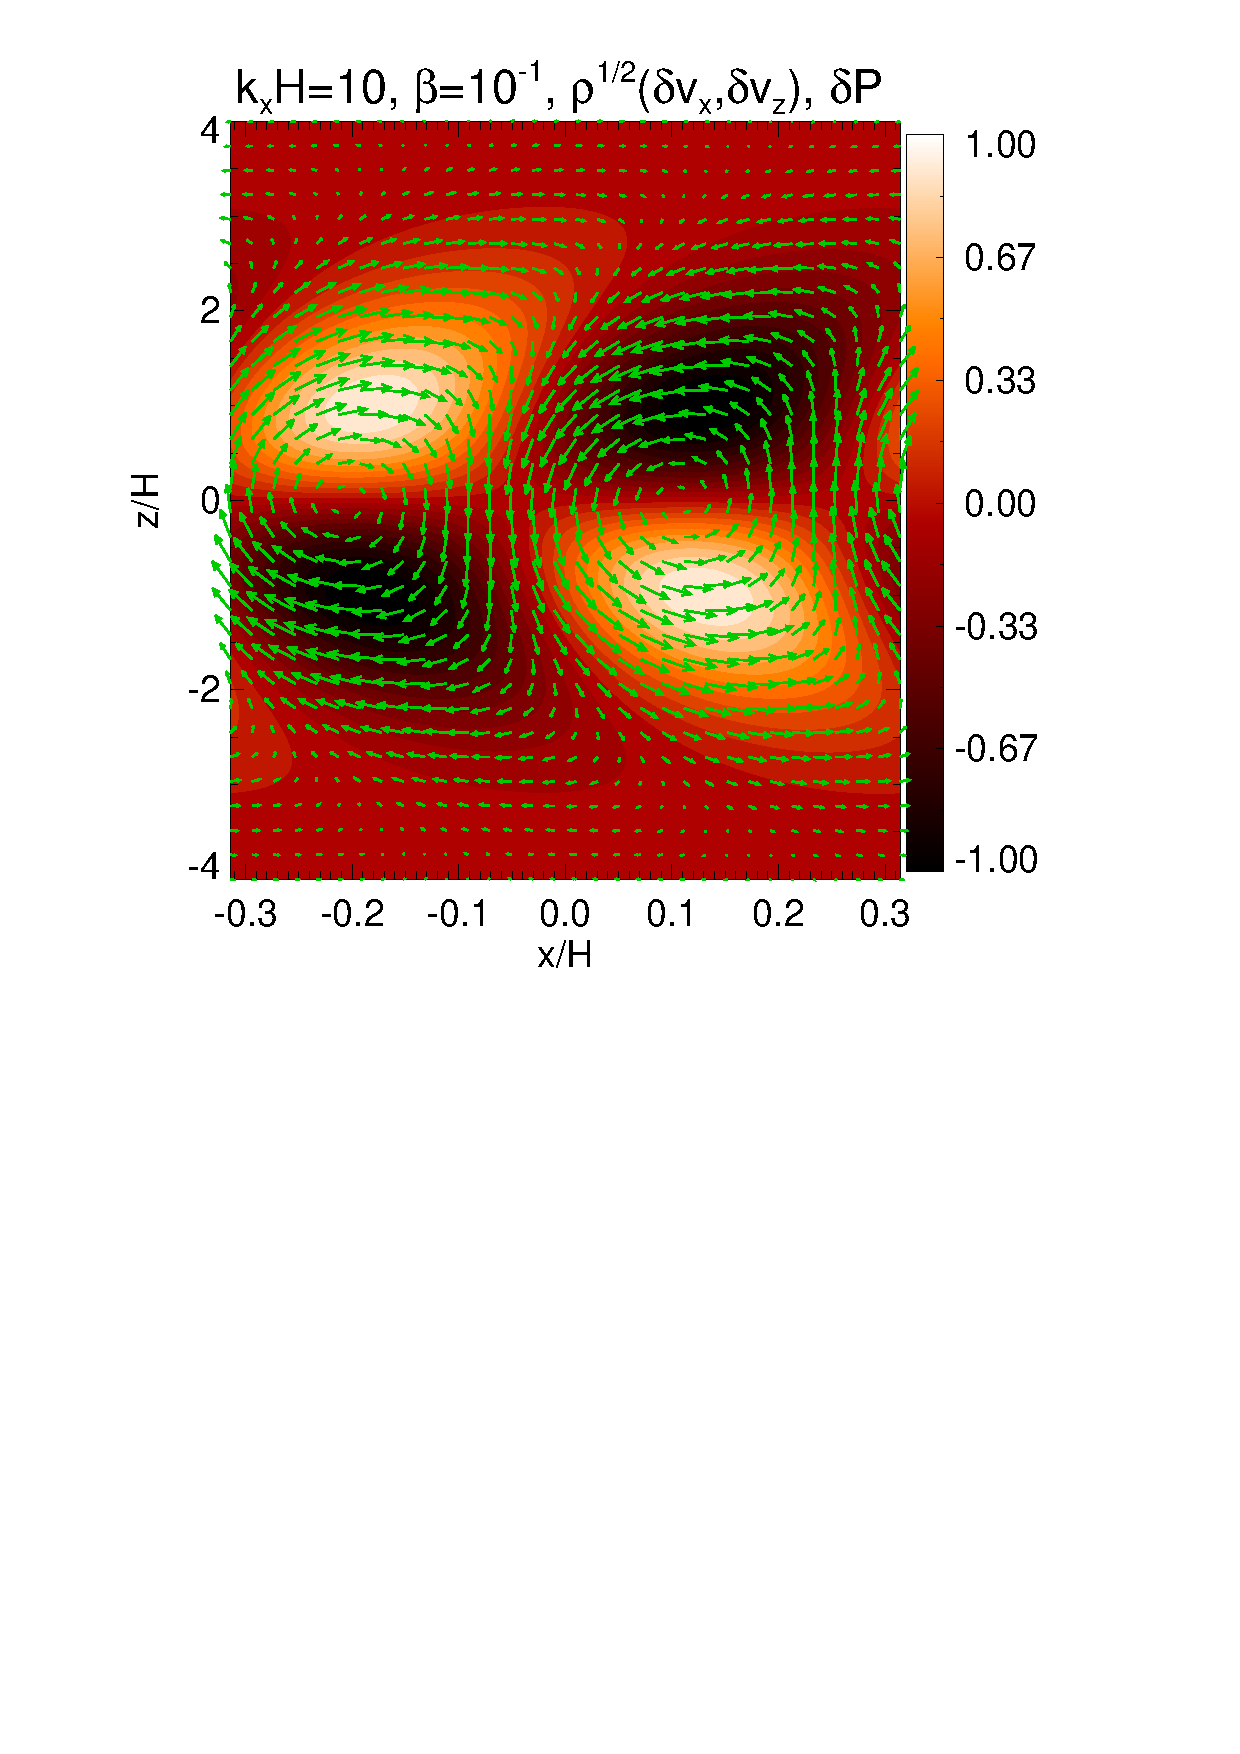
\includegraphics[width=\linewidth]{figures/result2d_cool}
  \caption{Same as  Fig. \ref{lowfreq_eigenfunc_2d} but with a thermal
    relaxation timescale $\beta=0.1$. 
    \label{lowfreq_eigenfunc_2d_cool}
  }
\end{figure}

Figures \ref{lowfreq_eigenfunc_cool} and \ref{lowfreq_eigenfunc_2d_cool}
illustrate the eigenfunction of the fundamental mode with $\khat=10$ and
$\beta=0.1$. Compared with the small $\beta$ case in 
Figs. \ref{lowfreq_eigenfunc} and \ref{lowfreq_eigenfunc_2d}, the eigenfuctions 
show a more complex variation of phase with height.  This dependence yields 
the `tilted' appearance of pressure field in  Fig. \ref{lowfreq_eigenfunc_2d_cool}.
Physically, the increased role of buoyancy, which increases with height, explains 
why larger $\beta$ values produce more complex vertical structure. 

\begin{figure}
 % \includegraphics[width=\linewidth,clip=true,trim=0cm 1.75cm 0cm
  %0cm]{figures/compare_modes_cool_kx30_z3_analytic.ps} 
  \includegraphics[width=\linewidth,clip=true,trim=0cm 1.75cm 0cm
  0cm]{figures/compare_modes_cool_kx30_z5_analytic.ps}
  \includegraphics[width=\linewidth]{figures/compare_modes_cool_kx30_z7_analytic.ps}
  \caption{Same as Fig. \ref{compare_modes_cool_kx10} but for
    $\khat=30$ and domain sizes $\zmax = 5H$ (\emph{top}) and $7H$ (\emph{bottom}). Examples of surface modes are marked with `s'. 
    \label{compare_modes_cool_kx30} 
  }
\end{figure}

Fig. \ref{compare_modes_cool_kx30} shows how cooling affects higher wavenumber
modes, specifically $\khat=30$.   We only show the larger domains with $\zmax = 5H, 7H$. 
These cases again show good convergence for $\beta \geq 0.03$, which the
the smaller domain with  $\zmax = 3H$ lacks.

With slower cooling, the wave frequency shows a more complex 
dependence on mode order, both analytically and numerically. For $\beta = 0.1$,
 the fundamental mode (which lies on the $M = 0$ curve) no longer has the smallest $|\omega|$ value.  

Moreover, the fundamental mode is no longer the fastest growing mode for $\beta \geq 0.03$, or even 
for $\beta = 0.1$.  This complication is not actually surprising since $|hq\khat| = 1.5$ is no longer less than unity,
as required in the analytic derivation of \S\ref{iso_vsi_beta_crit}.  Though  inconvenient,  given that the 
fundemental mode is easy to identify and the most numerically converged, this complication is not ultimately significant
for the operability of the VSI.  

Fig. \ref{compare_modes_cool_kx30} also demonstrates that artificial surface modes are damped for $\beta \geq 0.03$.
We are thus confident that artificial surface modes should not affect our determination of the critical cooling time.


%For clarity, we only plot analytic results 
%for the fundamental mode ($M=0$) and $M=1,\,2$, and omit the 
%squares. The fundamental mode is again insensitive to $\zmax$ and are
%in close agreement with analytic results. However, 
%there is increasing mismatch between analytical and numerical results
%for higher order modes as $\beta$ is increased. This suggests that, in
%the presence of buoyancy, boundary effects become important for these
%modes, which have larger $\khat$ than that considered previously. For
%example, for $\zmax=5H$ and $\zmax=7H$, we 
%find modes slightly more unstable than the fundamental
%mode even when $\beta=0.1$ (the leftmost eigenvalues in the lower two
%panels), but these are clearly affected by boundary
%conditions as they are absent for $\zmax=3H$. 
%
%Nevertheless, as before we observe more effective stabilization for
%higher order modes, including the absence of surface modes, for
%example as $\beta$ is increased from $0.01$ to $0.03$ (for $\zmax\geq
%5H$). 

\begin{figure}
  %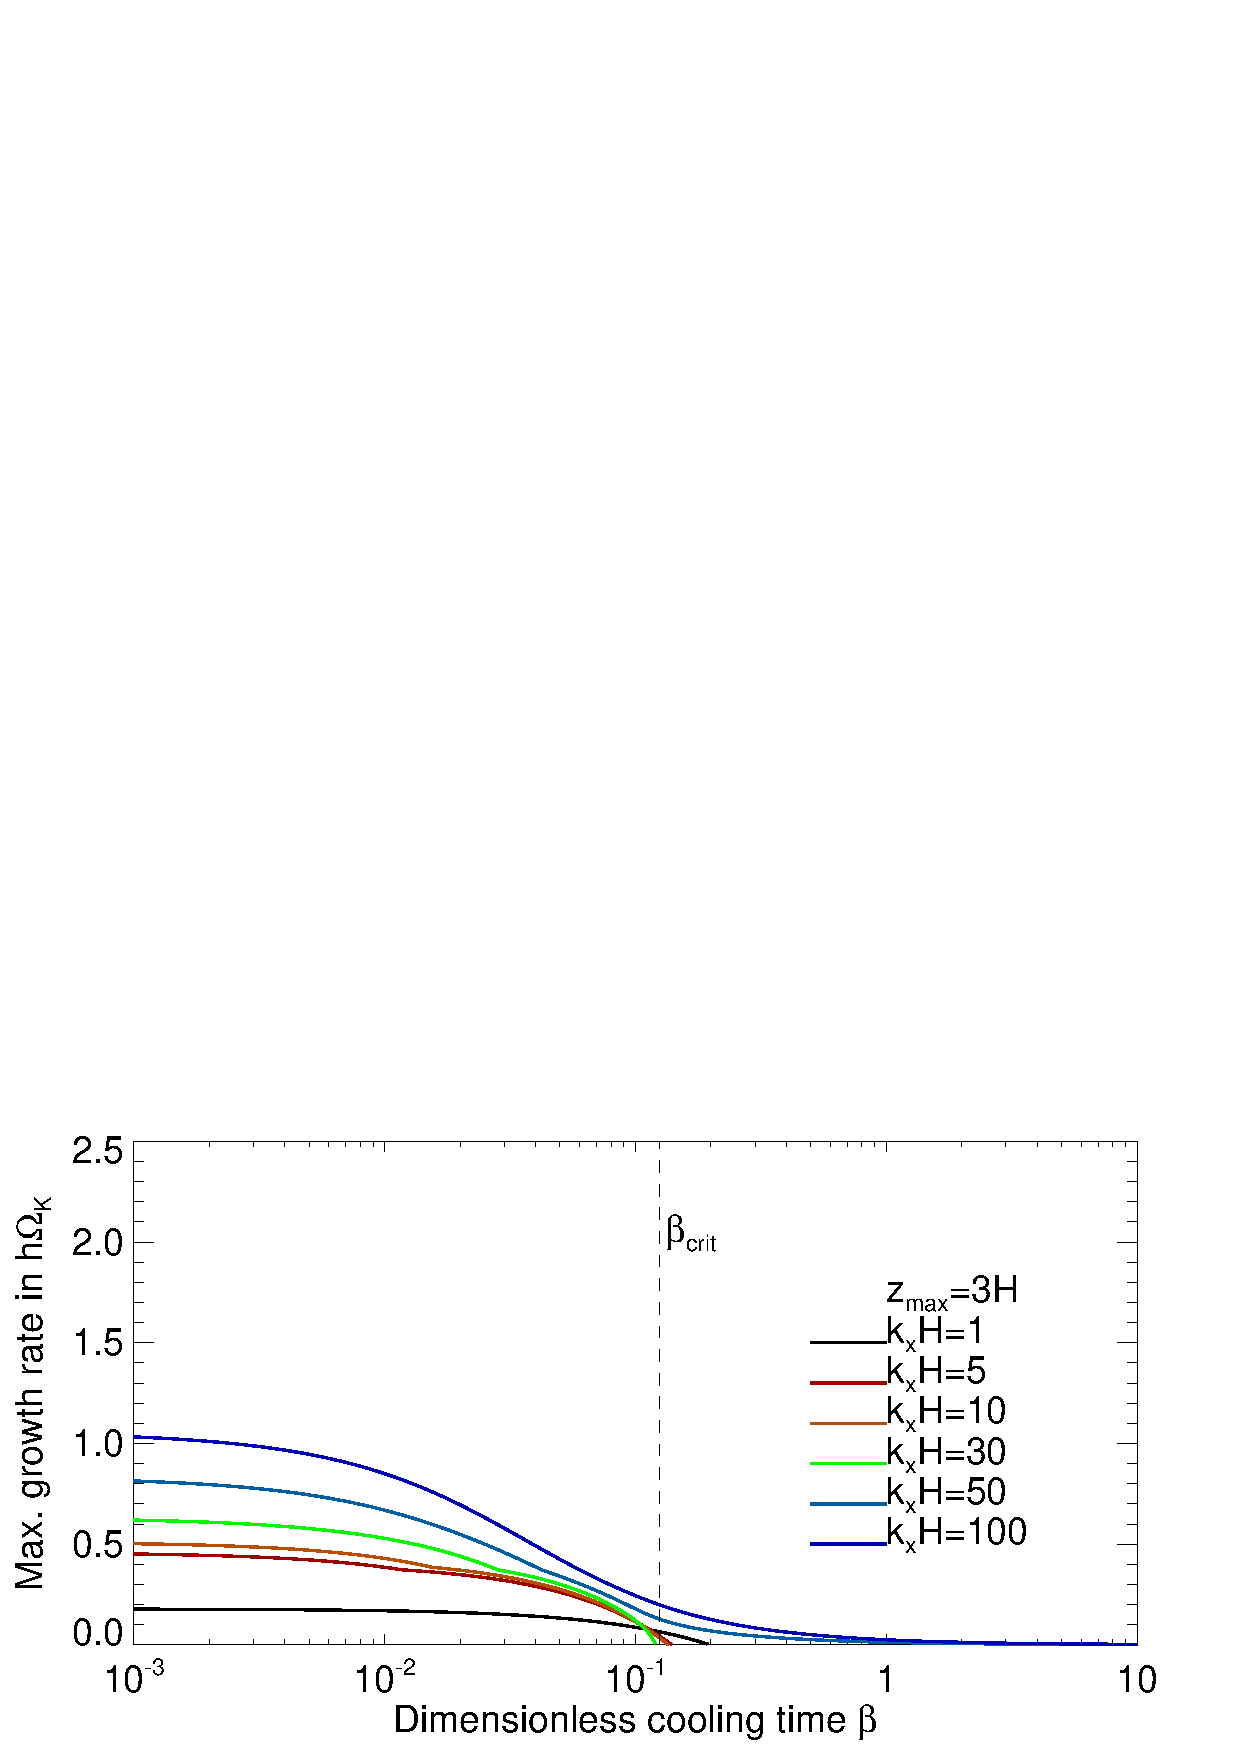
\includegraphics[width=\linewidth,clip=true,trim=0cm 1.75cm 0cm
  %0.9cm]{figures/gcorr_compare_iso_maxrate_z3} 
  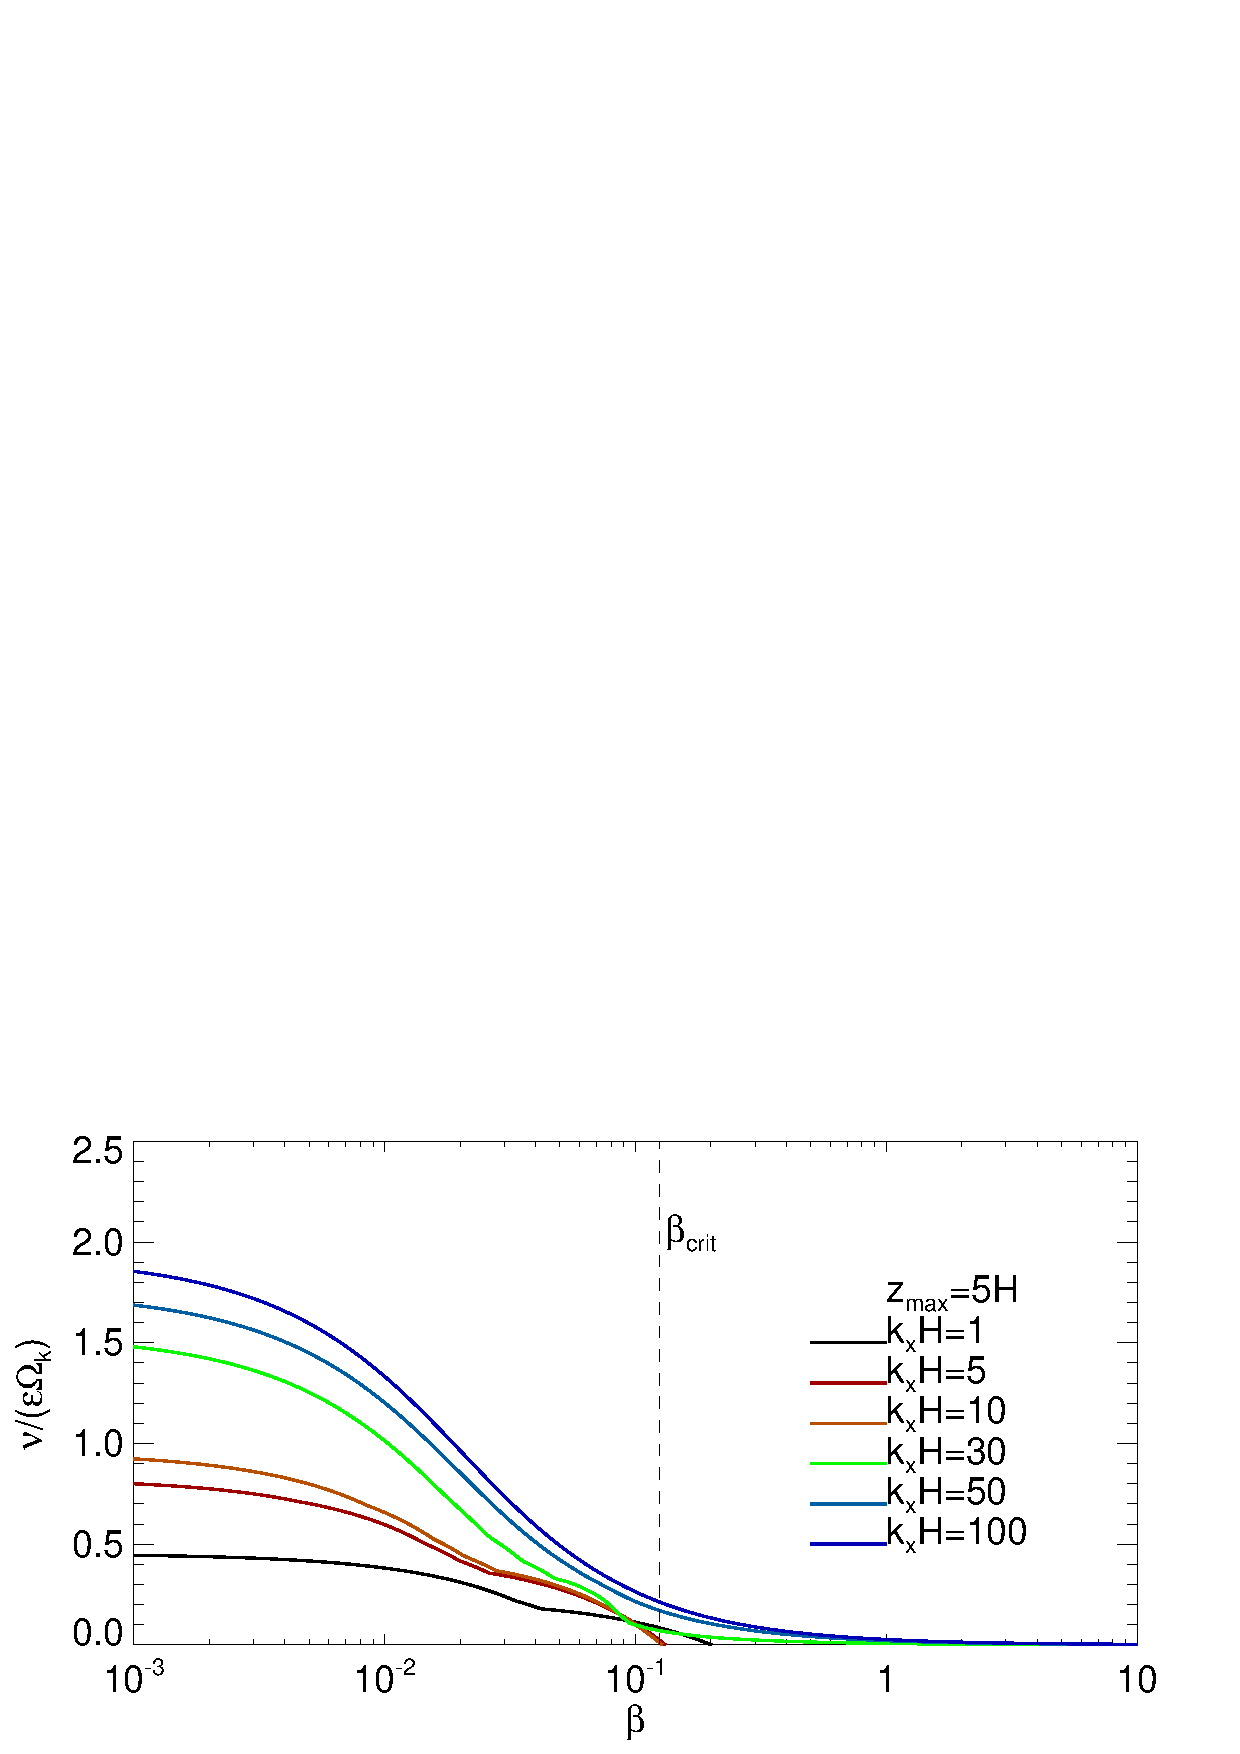
\includegraphics[scale=0.4415,clip=true,trim=0cm 1.75cm 0cm
  0.9cm]{figures/gcorr_compare_iso_maxrate_z5} 
  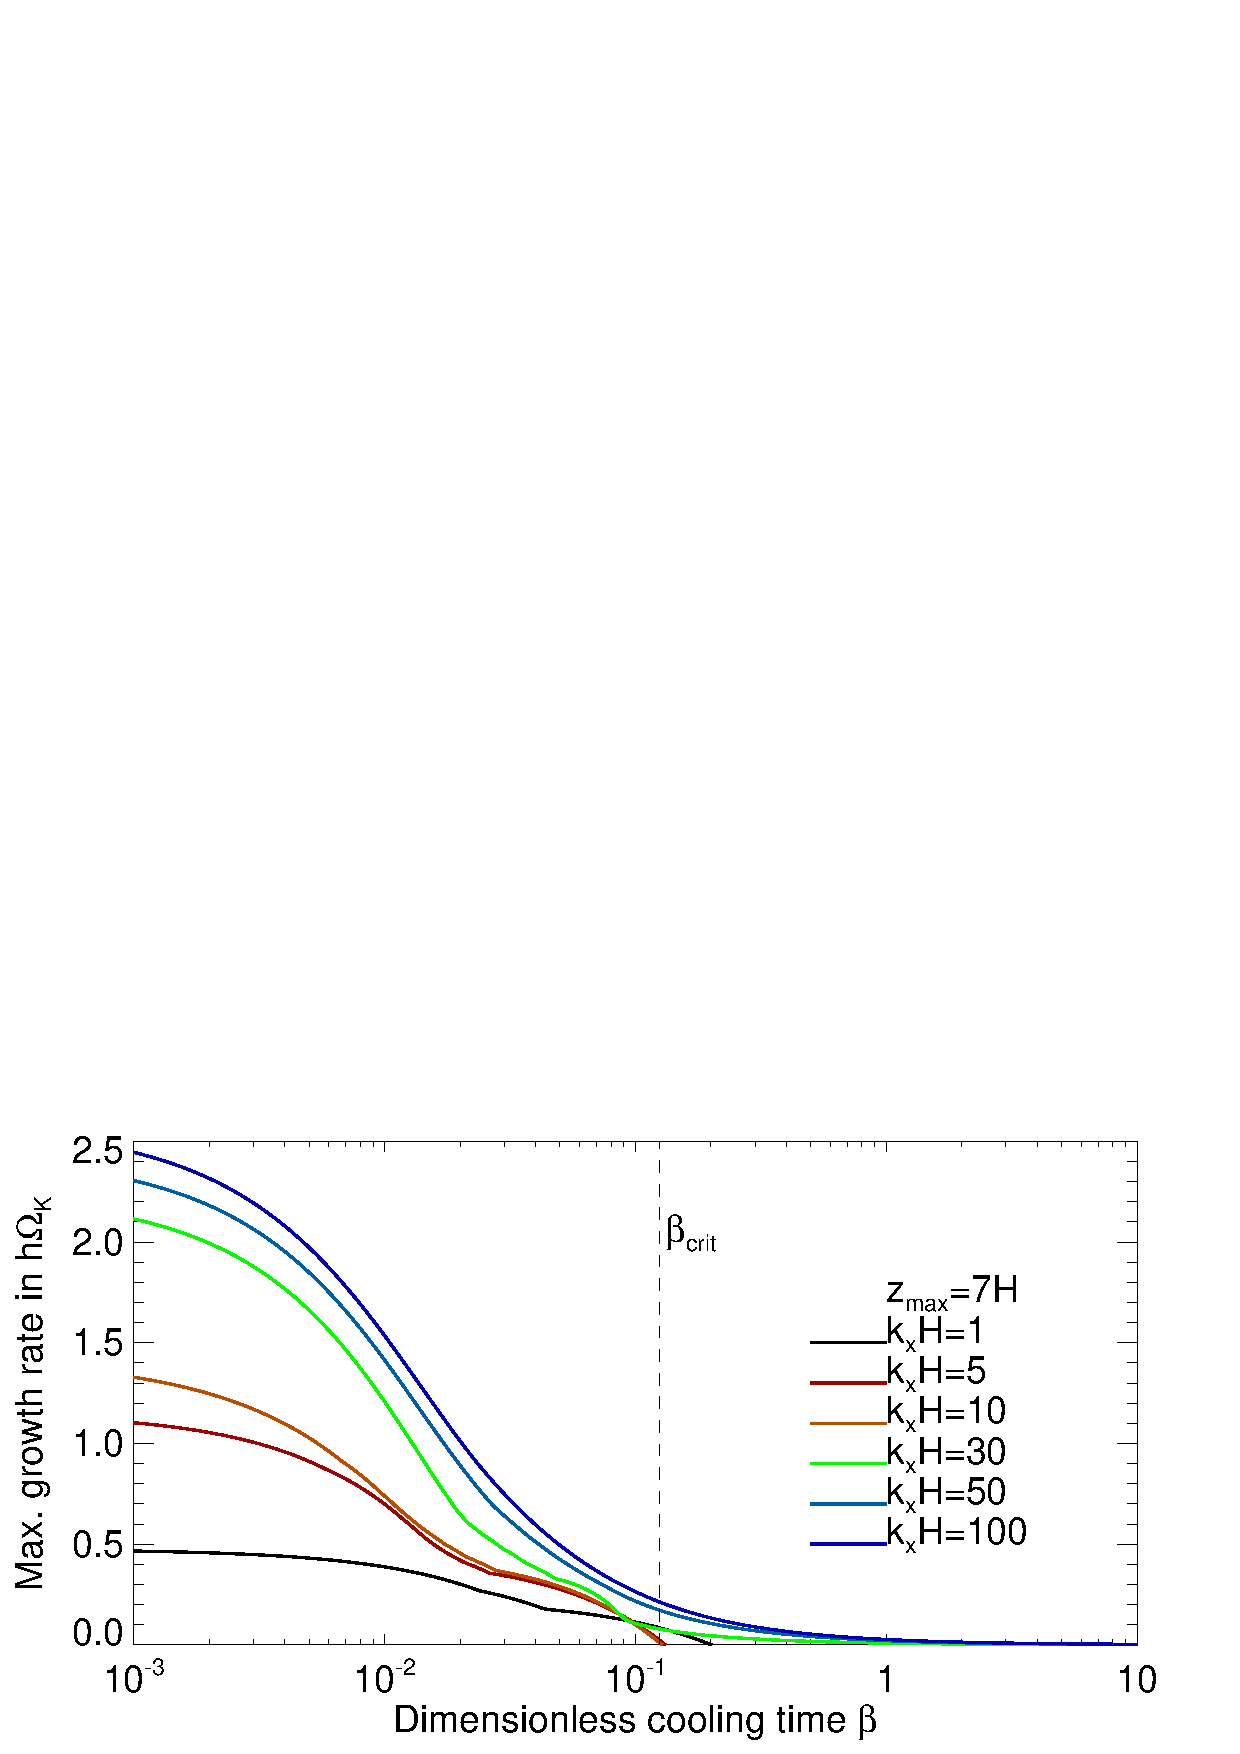
\includegraphics[scale=0.4415,clip=true,trim=0cm 0.0cm 0cm
  0.9cm]{figures/gcorr_compare_iso_maxrate_z7}  
  \caption{Maximum VSI growth rates in the fiducial disk 
     model as a function of the thermal relaxation timescale
     $\beta$, for %$\zmax=3H$ (top), 
     $\zmax=5H$ (top) and $\zmax=7H$ (bottom). The vertical line is the
     critical thermal timescale $\beta_\mathrm{crit}$ obtained  
     from Eq. \ref{iso_vsi_cond}. 
     \label{bcrit_compare1}}   
 \end{figure} 


\subsection{Critical thermal relaxation timescale}\label{bcrit_num_test}
Having explored the behavior of VSI modes with cooling, we turn to the numerical validity of the 
analytic cooling criterion for vertically isothermal disks, $\beta < \beta_\mathrm{crit} = h|q|/(\gamma -1)$.

Fig. \ref{bcrit_compare1} shows how VSI growth rates vary with cooling time 
in our fiducial model with $\beta_\mathrm{crit} = 0.125$.  
Curves are for a fixed horizontal wavenumber, and show the maximum growth rate for all vertical mode orders.  The 
discontinuity in some curves occurs when the fastest growth switches to a different mode order.

For $\khat = 5, 10$, the growth rate drops to zero at the expected $\beta = \beta_\mathrm{crit}$.
For longer wavelength modes, with $\khat = 1$, growth persists to slightly longer cooling times.  
This difference is not surprising since our analytic derivation assumed $\khat^2 \gg1$, and 
the change is quantitatively minor.

For shorter wavelengths, with $\khat \geq 30$, growth persists for $\beta$ significantly larger
than $\beta_\mathrm{crit}$.  This tail of growth is partly explained by the breaking of the $\khat < 1/|qh| = 20$ 
approximation, used in  the analytic derivation.  Despite the lack of a clear stability boundary 
at high $\khat$, the $\beta_\mathrm{crit}$ threshold remains useful, since growth rates drop to 
$\lesssim 10\%$ of  their maximum value at  $\beta_\mathrm{crit}$ and continue to fall for larger $\beta$. 
 Moreover, we expect that longer wavelength modes with $\khat \lesssim 20$
are more significant for disk transport, see \S\ref{caveats_visc}.

Comparing the $\zmax/H = 5, 7$ cases in Fig. \ref{bcrit_compare1}, we see that the location of the vertical
boundary has little effect on the critical cooling time.  This agreement occurs despite the fact that peak growth rates
differ as $\beta \to 0$.  We are thus confident that artificial boundary effects, including surface modes, do not
affect our analysis of the critical cooling time.

Our results agree with the vertically isothermal analysis of \citetalias{nelson13} 
which used the same disk parameters as our fiducial model.  The expected $\beta_\mathrm{crit} = 0.125$ 
is consistent with the simulations shown in their Fig.\ 12.  \citetalias{nelson13}  
found nonlinear VSI growth for $\beta = 0.06< \beta_\mathrm{crit}$ but no growth for 
  $\beta = 0.6 > \beta_\mathrm{crit}$.\footnote{Since the dimensionless cooling time $T_{\rm relax}$ in \citetalias{nelson13}
  is normalized to the orbital period, we convert $\beta = \OmK P_{\rm orb} T_{\rm relax} = 2 \pi T_{\rm relax}$.}

\begin{figure}
  \includegraphics[width=\linewidth,clip=true,trim=0cm 0.cm 0cm
  0cm]{figures/bcrit_compare_q.ps} 
  \includegraphics[width=\linewidth,clip=true,trim=0cm 0.0cm 0cm
  0.8cm]{figures/bcrit_compare_g.ps}
  \includegraphics[width=\linewidth,clip=true,trim=0cm 0.0cm 0cm
  0.8cm]{figures/bcrit_compare_e.ps} 
  \caption{Dependence of the upper limit to the thermal relaxation timescale
    $\beta_\mathrm{crit}$ for the fundamental VSI mode on disk
    parameters. The fiducial setup is $(\gamma, \Gamma= (1.4, 1.011)$
    and $(p,q, h)=(-1.5,-1,0.05)$. Top: varying 
    $q\in[-1.2,-0.2]$; middle: varying $\gamma\in[1.2,2.0]$; bottom:
    varying $ h\in[0.02,0.1]$. The perturbation wavenumber is
    $\khat=10$.  
    \label{bcrit_compare}}  
\end{figure}

Fig.\ \ref{bcrit_compare} confirms that the numerically determined
$\beta_\mathrm{crit}$ shows the expected scaling with disk parameters $h$, $q$, and $\gamma$.
For this test we fix $\khat = 10$ (an appropriate value for all the reasons discussed above) and measure
the smallest $\beta$ value where growth vanishes.  The agreement with the analytic scaling of 
Eq.\ \ref{iso_vsi_cond} is quite good, confirming the applicability of our critical cooling time in
vertically isothermal disks.


%we plot the maximum VSI growth rates
%found in the fiducial disk model as a function of the thermal
%relaxation timescale $\beta$ for several values of $\khat$ and
%$\zmax$. We also plot the critical timescale
%$\beta_\mathrm{crit}=0.125$ for the fiducial disk parameters.   
%
%Note that the curves are not neccessarily smooth because the most unstable
%mode may not always correspond to the same type of disturbance. For example,
%as seen above, for $\khat \leq 10$ higher order body modes are
%dominant as $\beta\to 0$, but the fundamental 
%mode becomes dominant as $\beta$ is increased. For $\khat=1$ the VSI
%can operate slightly beyond $\beta_\mathrm{crit}$  (recall that
%$\beta_\mathrm{crit}$ was derived assuming $\khat^2\gg 1$). For
%$\khat=5,\,10$ (and $30$ for $\zmax=3H$), we find
%$\beta_\mathrm{crit}$ accurately predicts the thermal timescal beyond
%which the VSI is suppressed.   
%
%Complications from vertical boundaries arise when considering large
%$\khat$. For $\khat=30$ and $\zmax=5H,\,7H$ we find for $\beta\gtrsim
%0.1$ the dominant disturbance correspond to the leftmost eigenvalues 
%seen in the lower two panels of Fig. \ref{compare_modes_cool_kx30},
%which do not exist for $\zmax=3H$. For $\khat=50,\,100$ and
%$\beta\to0$, we find surface modes dominate so the maximum growth rate
%depends on $\zmax$ in the limit of rapid thermal relaxation. 
%However, the maximum growth rate is insensitive to 
%$\zmax$ for moderately large $\beta$ ($\gtrsim 0.1$), i.e. close to
%the stabilization of the fundamental mode.  


%Our result is consistent with numerical simulations performed by
%\citetalias{nelson13} for which a thermal relaxation timescale $\beta\gtrsim
%0.6$ stabilized the VSI; as Fig. \ref{bcrit_compare1} show that growth
%rates for $\beta\gtrsim 0.6$ are small, and are restricted to very
%small radial lengthscales $\sim 10^{-2}H$, for which current numerical
%simulations may not be able to resolve.
%
%As pointed out by \citetalias{barker15}, in vertically isothermal disks with
%an imposed boundary, surface modes are dependent on $\zmax$, but they
%are often the most unstable. Despite this caveat, and that surface
%modes are not accounted in our analysis, we see from
%Fig. \ref{bcrit_compare1} that $\beta_\mathrm{crit}$ nevertheless
%provides a reasonable estimate for an upper limit to the thermal
%timescale for the VSI.  
%
%We further  test the dependence of $\beta_\mathrm{crit}$ on disk parameters
%(Eq. \ref{iso_vsi_cond}).  We use the fiducial setup as a  reference
%point and vary $q\in[-0.2,-1.2]$,  $\gamma\in[1.2,2.0]$, and
%$ h\in[0.02,0.1]$ separately. The numerically obtained
%$\beta_\mathrm{crit}$ are shown in Fig. \ref{bcrit_compare} in
%comparison with Eq. \ref{iso_vsi_cond}, which generally agree. This
%result, together with Fig. \ref{bcrit_compare1}, shows that  
%$\beta \lesssim \beta_\mathrm{crit}$ is a practical
%criteria for the VSI to operate effectively in stably stratified,
%vertically isothermal disks.   

\subsection{Vertically non-isothermal disk model} 
We briefly examine a vertically non-isothermal disk model with 
a physical surface. Recall from Eq. \ref{vertical_shear_ex} that in
general the vertical shear rate $\p_z\Omega\propto s$, the radial
entropy gradient. From the expression for the critical cooling timescale,
Eq. \ref{iso_vsi_cond}, it is reasonable to expect a similar criteria
for vertically non-isothermal disks in the form 
\begin{align}\label{bcrit_noniso}
 \beta_\mathrm{crit}\to\beta_\mathrm{crit, noniso} =
 \frac{h|s|}{\gamma - \Gamma}. 
\end{align}

Here, we consider a disk model with $(p,q, h)=(-0.5,-1,0.05)$ and $(\gamma,
\Gamma)=(1.4,1.3)$. We set the vertical domain size close to the
physical disk surface, $\zmax = 0.99H_s\simeq 2.6H$, which is smaller
than our standard domain size. For this setup, $s=-0.85$ and
$\beta_\mathrm{crit,noniso}=0.425$, which is $\sim 3$ times larger than
our fiducial, vertically isothermal disk with $\beta_\mathrm{crit}=0.125$. 

% A disk surface at finite height
% means that higher order body modes and surface modes are better
% defined (cf. in vertically isothermal disk models where the disk
% boundary $\zmax$ is a free parameter, see \citetalias{barker15}). 

In Fig. \ref{compare_modes_vnoniso_kx10} we plot the mode diagram for
$\khat=30$ for several values of $\beta$. This plot is 
qualitatively similar to Fig. \ref{compare_modes_cool_kx10}. As before
we find as $\beta$ is increased, higher order modes are rapidly
stabilized, eventually only the fundamental mode can operate before
the VSI is entirely suppressed. (Note the significant reduction in
growth rates for $\beta=0.4$, which is close to
$\beta_\mathrm{crit,noniso}$.) However, this behavior is not seen for 
large wavenumbers (see below). 

\begin{figure}
  \includegraphics[width=\linewidth,clip=true,trim=0cm 0cm 0cm
  0cm]{figures/compare_modes_Gam1.3_kx30.ps}
  \caption{Unstable modes in a vertically non-isothermal disk with
    $\khat=30$ and a range of thermal relaxation timescales.  
    \label{compare_modes_vnoniso_kx10}}
\end{figure} 

In Fig. \ref{bcrit_compare2} we plot the maximum VSI growth
rates in the vertically non-isothermal disk model, which is
qualitatively similar to Fig. \ref{bcrit_compare1} for the vertically
isothermal disk. For $\khat=O(10)$, there is a   
precise cut-off thermal timescale close to that given by
Eq. \ref{bcrit_noniso}. We found that very large wavenumbers, 
$\khat > O(10^2)$, were needed to enable surface modes, and modes with
such values of $\khat$ do not have a maximum cooling time. However,
these small lengthscales may not be important in practice
(see \S\ref{caveats_visc}). Thus, $\beta<\beta_\mathrm{crit,noniso}$ 
provides an excellent criteria for instability.   

\begin{figure}
  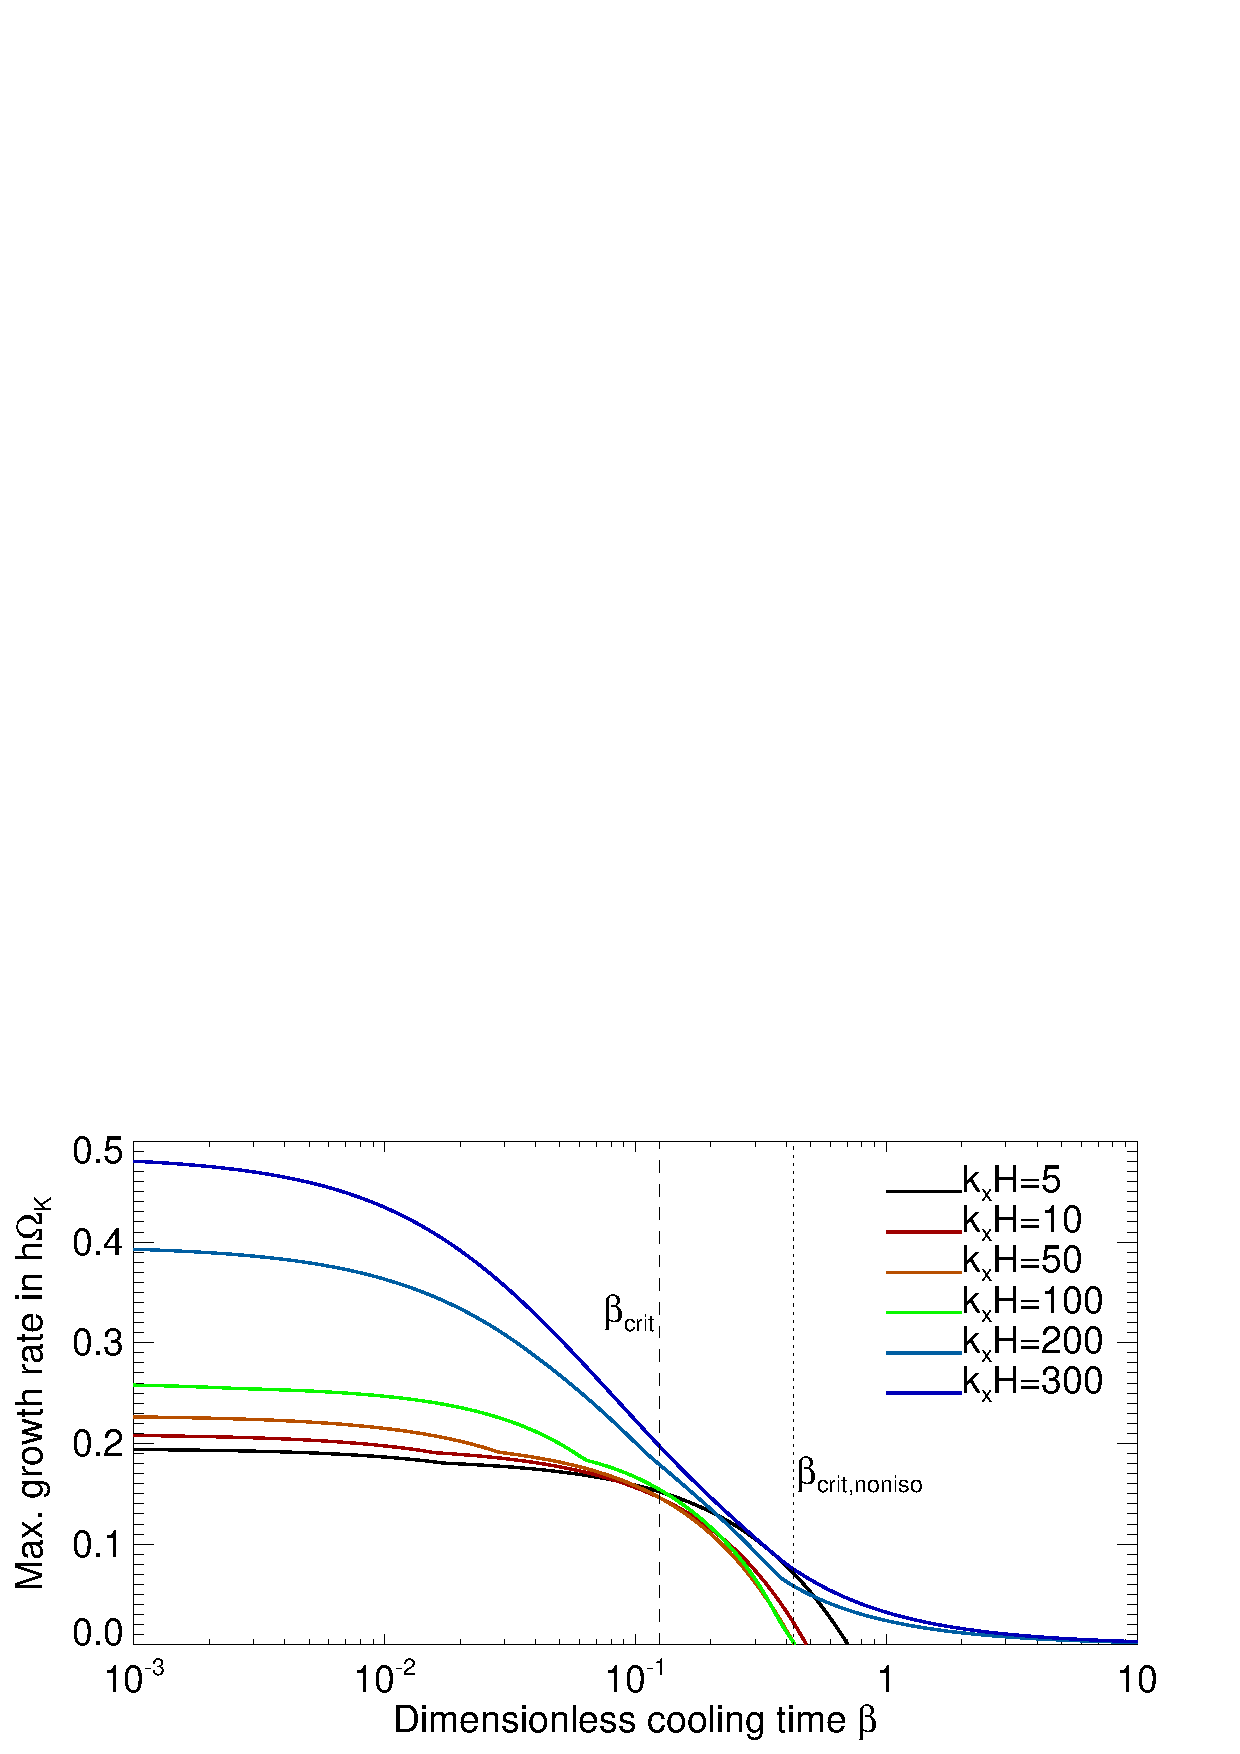
\includegraphics[scale=0.4415]{figures/gcorr_compare_vnoniso_maxrate2} 
  \caption{Maximum VSI growth rates in the vertically non-isothermal disk
    model as a function of the thermal relaxation timescale
    $t_c=\beta\OmK^{-1}$. The vertical dashed line is the critical thermal
    timescale given by Eq. \ref{iso_vsi_cond}. A conjectured critical thermal
    timescale accounting for a non-isothermal background, given by 
     $\beta_\mathrm{crit,noniso}= 0.425$ (see Eq. \ref{bcrit_noniso}),   
    is also shown as the vertical dotted line. 
    \label{bcrit_compare2}}   
\end{figure} 

The above calculation demonstrates that the effect of introducing
finite cooling on the VSI operates very similarly in vertically
isothermal disks with an imposed surface, and in vertically
non-isothermal disks with a physical surface. This is despite the fact
that the vertical buoyancy frequency, $N_z$, formally diverges as $|z|\to H_s$.  

% We briefly consider vertically non-isothermal disks with 
% $\Gamma=1.4$ and $(p,q, h)=(0,-1,0.05)$ as simulated in
% \cite{nelson13}. In this case we set $\zmax=0.99H_s$.  

% We do not find surface modes for $\khat=10$, but do find them for
% sufficiently large $\khat$. We demonstrate this in  % In the vertically
% % non-isothermal disk, surface modes develop for sufficiently large 
% % $\khat$ \citep{barker15}. We demonstrate them in
% Fig. \ref{compare_modes_vnoniso_kx100} which show eigenvalues for
% $\khat=100$. While growth rates generally decrease with increasing 
% $\beta$, we find eigenvalues can overlap, making it difficult to 
% distinguish between different modes. However, since there 
% is a well-defined surface, we may seek the  
% most unstable mode without the boundary-dependent issue that arose 
% with a vertically isothermal disk in the limit $\beta\to0$.  

% \begin{figure}
%   \includegraphics[width=\linewidth,clip=true,trim=0cm 0cm 0cm
%   0cm]{figures/compare_modes_Gam1.084_kx100.ps}
%   \caption{Same as Fig. \ref{compare_modes_vnoniso_kx10} but with
%     $\khat=100$. In this case surface modes appear nearly parallel to
%     the vertical axis
%     (cf. Fig. \ref{compare_modes_vnoniso_kx10}). However, this
%     distinction becomes difficult for increasing $\beta$ as modes
%     overlap. 
%     % but
%     % overlap with body modes (those that are roughly horizontal when 
%     % $\beta=10^{-3}$) as $\beta$ is further increased. 
%     \label{compare_modes_vnoniso_kx100}}
% \end{figure}

% Fig. \ref{compare_eigenvz_vnoniso_kx100} show the most unstable modes
% with $\khat=100$ and $\beta=10^{-3},\, 10^{-2}$ and
% $0.1$. For $\beta=10^{-3}$ the most 
% unstable mode is an asymmetric surface mode \citepalias[also seen in Fig. 7
% of][]{barker15}. However, increasing the thermal timescale to
% $\beta=10^{-2}$ an anti-symmetric surface mode becomes
% dominant. Further increasing to $\beta=0.1$, the dominant mode has a
% mixed character between a surface mode and the fundamental
% mode. Notice as $\beta$ is increased the perturbation amplitude near
% the vertical boundaries become negligible. This is not surprsing since  
% the stabilizing effect of buoyancy is largest at the disk surface. 
% %formally diverges 

% \begin{figure}
%   \includegraphics[width=\linewidth,clip=true,trim=0cm 1.73cm 0cm
%   0cm]{figures/eigenvectorvz_vnoniso_kx100_beta0d001.ps}
%   \includegraphics[width=\linewidth,clip=true,trim=0cm 1.73cm 0cm
%   0cm]{figures/eigenvectorvz_vnoniso_kx100_beta0d01.ps}
%   \includegraphics[width=\linewidth,clip=true,trim=0cm 0cm 0cm
%   0cm]{figures/eigenvectorvz_vnoniso_kx100_beta0d1.ps}
%   \caption{Vertical velocity eigenfunction of the most unstable mode
%     with $\khat=100$ found in the vertically non-isothermal disk with
%     $\beta = 10^{-3}$ (top), $\beta=10^{-2}$ (middle) and $\beta=0.1$
%     (bottom). 
%     \label{compare_eigenvz_vnoniso_kx100}}
% \end{figure}

% Fig. \ref{gcorr_compare_vnoniso} plots the fundamental VSI growth
% rates as a function of $\beta$ for $\gamma\in[1.4,2.5]$. In agreement
% with \citeauthor{nelson13}, in   
% the neutrally-stratified case $\gamma=\Gamma$ the disk is unstable 
% even for $\beta\gg 1$. This is due to the absence of a stabilizing
% vertical entropy gradient ($N_z^2\equiv 0$). % (Note that in the adiabatic limit 
% % this disk can be unstable according to the
% % Solberg-Hoiland criterion, Eq. \ref{solberg2}.) 

% For $\gamma>\Gamma$, i.e. stably stratified disks,
% Fig. \ref{gcorr_compare_vnoniso} shows that introducing finite thermal
% relaxation rapidly stabilizes the disk, similar to that observed for
% nearly vertically isothermal disks (Fig. \ref{bcrit_compare1}). For
% $\gamma=1.7,\,2.0,\,2.5$, growth rates reach zero at
% $\beta\simeq0.17,\,0.083,\,0.045$, respectively. Interestingly, these
% values are equal to $ h|q|/(\gamma-\Gamma)$. This suggests that
% the critical thermal relaxation timescale for vertically
% non-isothermal disks can also be estimated by Eq. \ref{iso_vsi_cond}
% but with $\gamma-1$ replaced by $\gamma-\Gamma$. 

% \begin{figure}
%   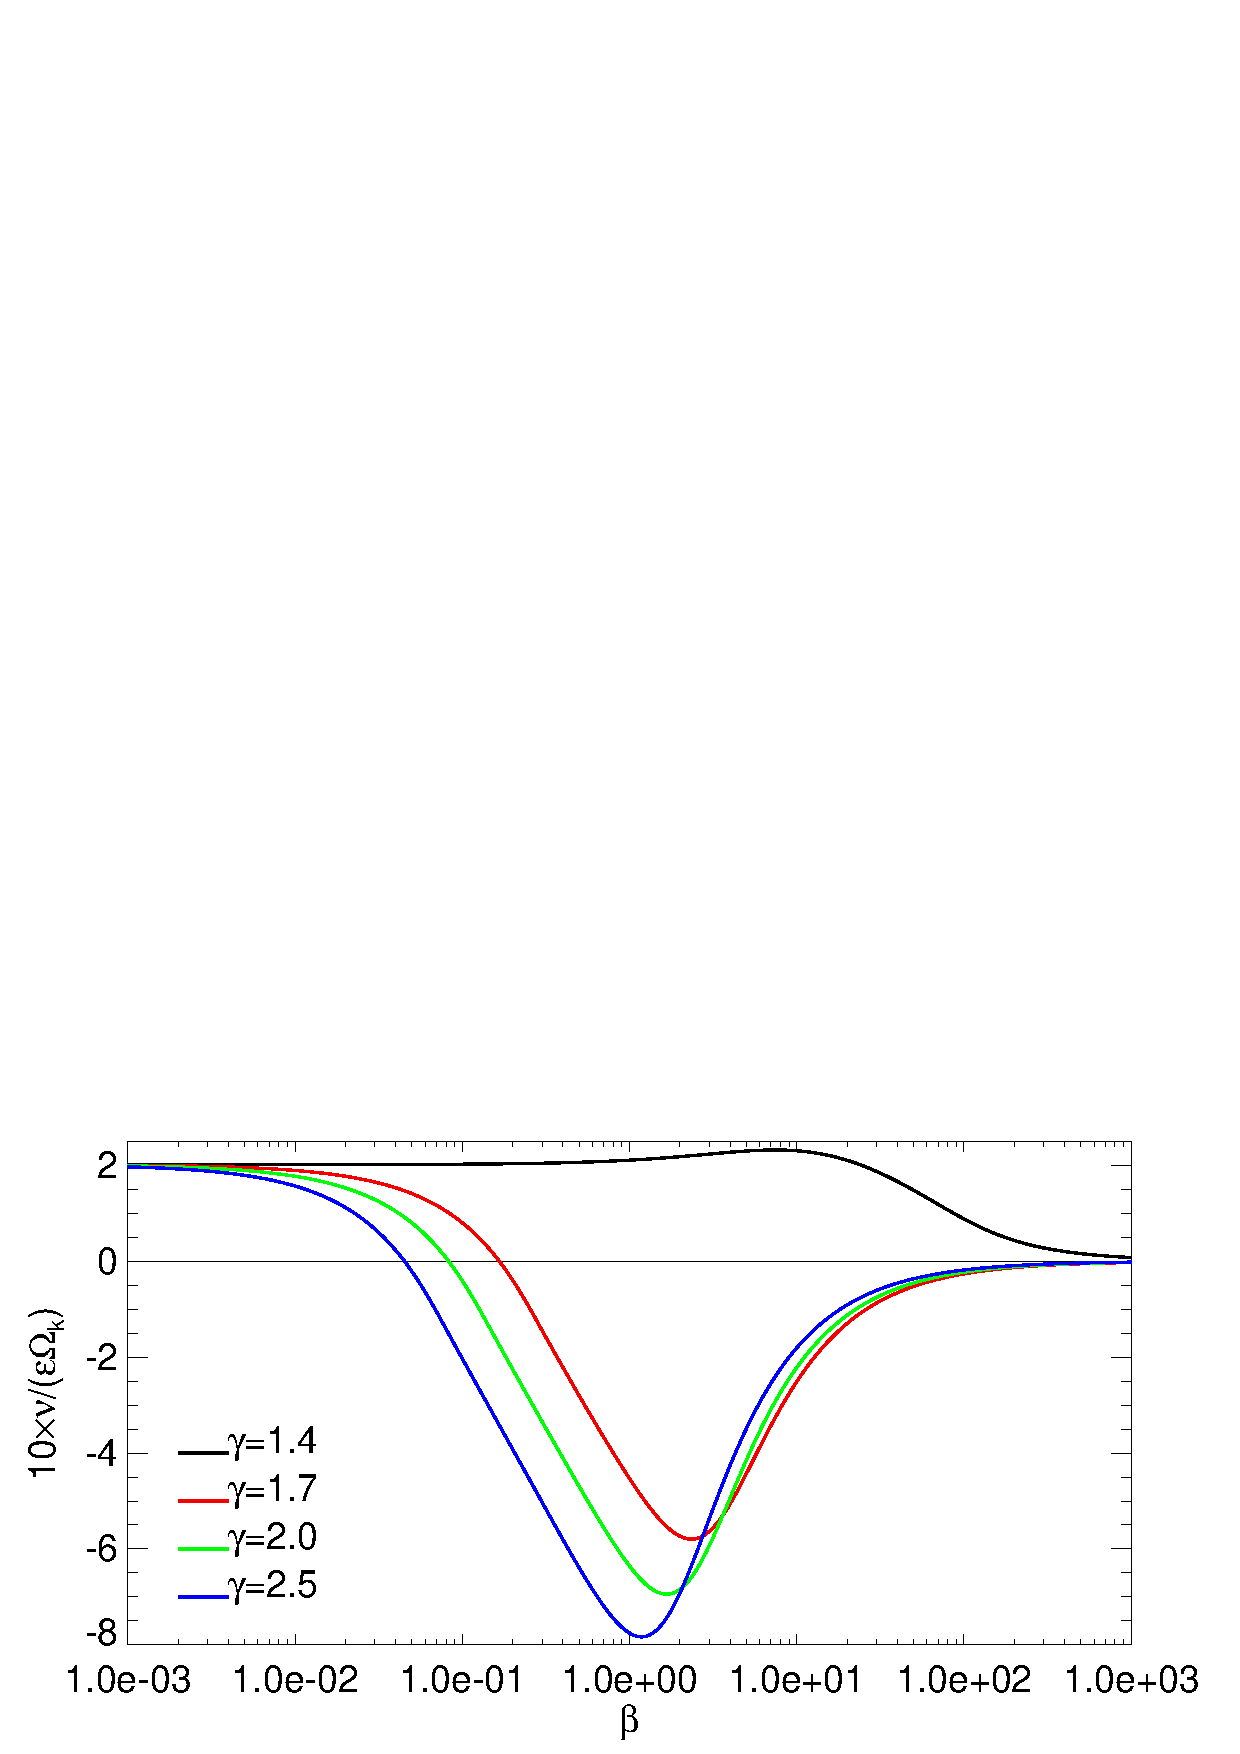
\includegraphics[width=\linewidth,clip=true,trim=0cm 0cm 0cm
%   0cm]{figures/gcorr_compare_vnoniso2}
%   \caption{Growth rate of the fundamental VSI mode as a function of
%     the thermal relaxation timescale $\beta$, in vertically
%     non-isothermal disks with $\Gamma=1.4$ and
%     $\gamma\in[1.4,2.5]$. The disk is neutrally
%     stratified for $\gamma=1.4$ and stably stratified for
%     $\gamma>1.4$. Other disk parameters are
%     $(p,q, h)=(0,-1,0.05)$ and the perturbation wavenumber is
%     $\khat=30$.   
%     \label{gcorr_compare_vnoniso}}
% \end{figure}












